\documentclass[12pt,twoside,onecolumn]{IEEEtran}
%\usepackage{times}
%\documentclass[12pt]{article}
\usepackage{epsfig, bbm, subfigure} % capt-of,ifthen, calc,
%\usepackage[mathbf,mathcal]{euler}
%\usepackage{pifont,epsfig}
\usepackage[
pdfauthor={Hari Sundar},
pdftitle={ Ph.D Proposal },
pdfcreator={pdftex},
pdfsubject={Computer Aided Diagnosis of Cardiomyopathies},
pdfkeywords={Cardiomyopathy, CAD, registration},
pagebackref  = {true},
hyperindex = {true},
colorlinks = {true},
linkcolor = {blue},
pagecolor = {blue},
citecolor = {blue}
]{hyperref} 
%\usepackage{cite}

\usepackage{amsmath}
\usepackage{algorithmic}
\usepackage{algorithm}
%\renewcommand{\baselinestretch}{1.5}
%\newcommand{\remove}[1]{}
\renewcommand{\div}{{\boldsymbol{\nabla}}}
% \overrideIEEEmargins

\newcommand{\ul}{\underline}
\newcommand{\bea}{{\begin{eqnarray}}}
\newcommand{\eea}{{\end{eqnarray}}}
\newcommand{\beq}{{\begin{equation}}}
\newcommand{\eeq}{{\end{equation}}}
\newcommand{\tmccrap}{These results are based upon a test version of the
Thinking Machines Corporation software where the emphasis was on providing
functionality and the tools necessary to begin testing the CM-5 vector units.
This software release has not had the benefit of optimization or performance
tuning and, consequently, is not necessarily representative of the performance
of the full version of this software.}
\newcommand{\tafsm}{T\,\includegraphics[width=0.75em]{logo-star.eps}\,AFSM}

\newfont{\amsbold}{msbm10}
\newfont{\logobold}{logobf10 scaled\magstep2}
\newcommand{\real}{\mathbb{R}}
\newcommand{\assembly}{\mathop{\mbox{\logobold A}}}
\def\nsd{{n_\mathrm{sd}}}
\def\isd{{i_\mathrm{sd}}}
\def\nen{{n_\mathrm{en}}}
\def\nel{{n_\mathrm{el}}}
\def\iel{{i_\mathrm{el}}}
\def\nln{{n_\mathrm{ln}}}
\def\nq{{n_\mathrm{eq}}}
\def\nelem{{n_\mathrm{e}}}
\def\nnode{{n_\mathrm{n}}}
\def\ndf{{n_\mathrm{dof}}}
\def\idf{{i_\mathrm{dof}}}
\def\ned{{n_\mathrm{ed}}}
\def\nee{{n_\mathrm{ee}}}
\def\iee{{i_\mathrm{ee}}}
\def\nint{{n_\mathrm{int}}}
\def\nquad{{n_\mathrm{quad}}}
\def\iquad{{i_\mathrm{quad}}}
\def\neemax{n_\mathrm{ee\_max}}
\def\npes{{n_\mathrm{PEs}}}
\def\Ot{\Omega_t}
\def\Gt{\Gamma_t}
\def\On{\Omega_n}
\def\Gn{\Gamma_n}
\newcommand{\Reynolds}{\mathrm{Re}}
\newcommand{\Prandtl}{\mathrm{Pr}}
\newcommand{\Froude}{\mathrm{Fr}}
\newcommand{\Strouhal}{\mathrm{St}}
\def\sbn{{\pmb n}}
\def\sbt{{\pmb t}}
\def\sbb{{\pmb b}}
\newcommand{\ba}{\mathbf{a}}
\newcommand{\bb}{\mathbf{b}}
\newcommand{\bc}{\mathbf{c}}
\newcommand{\bd}{\mathbf{d}}
\newcommand{\be}{\mathbf{e}}
\newcommand{\force}{\mathbf{f}}
\newcommand{\bg}{{\boldsymbol{\mathit{g}}}}
\newcommand{\bh}{{\boldsymbol{\mathit{h}}}}
\newcommand{\bi}{\mathbf{i}}
\newcommand{\bj}{\mathbf{j}}
\newcommand{\bk}{\mathbf{k}}
\newcommand{\bm}{\mathbf{m}}
\newcommand{\bn}{\mathbf{n}}
\newcommand{\bp}{\mathbf{p}}
\newcommand{\bq}{\mathbf{q}}
\newcommand{\br}{\mathbf{r}}
\newcommand{\bs}{\mathbf{s}}
\newcommand{\bt}{\mathbf{t}}
\newcommand{\bu}{\mathbf{u}}
\newcommand{\bv}{\mathbf{v}}
\newcommand{\bw}{\mathbf{w}}
\newcommand{\bx}{\mathbf{x}}
\newcommand{\by}{\mathbf{y}}
\newcommand{\bz}{\mathbf{z}}
\newcommand{\bA}{\mathbf{A}}
\newcommand{\bB}{\mathbf{B}}
\newcommand{\bC}{\mathbf{C}}
\newcommand{\bD}{\mathbf{D}}
\newcommand{\bE}{\mathbf{E}}
\newcommand{\bF}{\mathbf{F}}
\newcommand{\bG}{\mathbf{G}}
\newcommand{\bH}{\mathbf{H}}
\newcommand{\bI}{\mathbf{I}}
\newcommand{\bJ}{\mathbf{J}}
\newcommand{\bK}{\mathbf{K}}
\newcommand{\bL}{\mathbf{L}}
\newcommand{\bM}{\mathbf{M}}
\newcommand{\bN}{\mathbf{N}}
\newcommand{\bO}{\mathbf{O}}
\newcommand{\bP}{\mathbf{P}}
\newcommand{\bQ}{\mathbf{Q}}
\newcommand{\bR}{\mathbf{R}}
\newcommand{\bS}{\mathbf{S}}
\newcommand{\bT}{\mathbf{T}}
\newcommand{\bU}{\mathbf{U}}
\newcommand{\bV}{\mathbf{V}}
\newcommand{\bW}{\mathbf{W}}
\newcommand{\bX}{\mathbf{X}}
\newcommand{\bY}{\mathbf{Y}}
\newcommand{\bZ}{\mathbf{Z}}
\newcommand{\zero}{\mathbf{0}}
\newcommand{\bxi}{{\boldsymbol{\xi}}}
\newcommand{\balpha}{{\boldsymbol{\alpha}}}
\newcommand{\bomega}{{\boldsymbol{\omega}}}
\newcommand{\bchi}{{\boldsymbol{\chi}}}
\newcommand{\btheta}{{\boldsymbol{\theta}}}
%\newcommand{\bChi}{{\boldsymbol{\Chi}}}
\newcommand{\bepsilon}{{\boldsymbol{\epsilon}}}
\newcommand{\bPsi}{{\boldsymbol{\Psi}}}
\newcommand{\bphi}{{\boldsymbol{\phi}}}
\newcommand{\bpi}{{\boldsymbol{\pi}}}
\newcommand{\design}{\balpha}
\def\but{{\bf u}_{,t}}
\def\bvt{{\bf v}_{,t}}
\def\ST{{{\cal S}^h_\bT}}
\def\VT{{{\cal V}^h_\bT}}
\def\SH{{{\cal S}^h_H}}
\def\VH{{{\cal V}^h_H}}
\def\Su{{{\cal S}^h_\bu}}
\def\Vu{{{\cal V}^h_\bu}}
\def\SU{{{\cal S}^h_\bU}}
\def\VU{{{\cal V}^h_\bU}}
\def\Sv{{{\cal S}^h_\bv}}
\def\Vv{{{\cal V}^h_\bv}}
\def\Sp{{{\cal S}^h_p}}
\def\Vp{{{\cal V}^h_p}}
\def\Sh{{{\cal S}^h_\phi}}
\def\Vh{{{\cal V}^h_\phi}}
\def\Sun{{(\Su)_n}}
\def\Vun{{(\Vu)_n}}
\def\SHn{{(\SH)_n}}
\def\VHn{{(\VH)_n}}
\def\SUn{{(\SU)_n}}
\def\VUn{{(\VU)_n}}
\def\Svn{{(\Sv)_n}}
\def\Vvn{{(\Vv)_n}}
\def\Spn{{(\Sp)_n}}
\def\Vpn{{(\Vp)_n}}
\def\Shn{{(\Sh)_n}}
\def\Vhn{{(\Vh)_n}}
\newcommand{\strain}{{\boldsymbol{\varepsilon}}}
\newcommand{\stress}{{\boldsymbol{\sigma}}}
\newcommand{\blambda}{{\boldsymbol{\lambda}}}
\renewcommand{\div}{{\boldsymbol{\nabla}}}
\newcommand{\sbg}{\bg}
\newcommand{\sbh}{\bh}
\newcommand{\btau}{\boldsymbol{\tau}}
\newcommand{\tauT}{{\tau_\mathrm{\scriptscriptstyle CONS}}}
\newcommand{\tauu}{{\tau_\mathrm{\scriptscriptstyle MOM}}}
\newcommand{\taup}{{\tau_\mathrm{\scriptscriptstyle CONT}}}
\newcommand{\taudc}{{\tau_\mathrm{\scriptscriptstyle DC}}}
\newcommand{\tauadv}{{\tau_\mathrm{\scriptscriptstyle ADV}}}
\newcommand{\tausupg}{{\tau_\mathrm{\scriptscriptstyle SUPG}}}
\newcommand{\taupspg}{{\tau_\mathrm{\scriptscriptstyle PSPG}}}
\newcommand{\taugls}{{\tau_\mathrm{\scriptscriptstyle GLS}}}
\newcommand{\tauglsa}{{\tau_\mathrm{\scriptscriptstyle GLS1}}}
\newcommand{\tauglsb}{{\tau_\mathrm{\scriptscriptstyle GLS2}}}
\newcommand{\oneovermu}{\frac{1}{2 \mu_{1}}}
\newcommand{\lamovermu}{\frac{\lambda}{2 \mu_{1}}}
\newcommand{\lsqovermu}{\frac{\lambda^{2}}{2 \mu_{1}}}
\newcommand{\hash}{{\includegraphics[width=0.1in]{x.ps}}}
\newcommand{\hashblue}{{\includegraphics[width=0.1in]{x-blue.ps}}}
\newcommand{\subhash}{{\includegraphics[width=0.06in]{x.ps}}}
\newcommand{\subhashblue}{{\includegraphics[width=0.06in]{x-blue.ps}}}
\newcommand{\upup}           {{\includegraphics[width=0.1in]{h.ps}}}
\newcommand{\upupblue}       {{\includegraphics[width=0.1in]{h-blue.ps}}}
\newcommand{\upupred}        {{\includegraphics[width=0.1in]{h-red.ps}}}
\newcommand{\upupmagenta}    {{\includegraphics[width=0.1in]{h-magenta.ps}}}
\newcommand{\subupup}        {{\includegraphics[width=0.1in]{h.ps}}}
\newcommand{\subupupblue}    {{\includegraphics[width=0.06in]{h-blue.ps}}}
\newcommand{\subupupred}     {{\includegraphics[width=0.06in]{h-red.ps}}}
\newcommand{\subupupmagenta} {{\includegraphics[width=0.06in]{h-magenta.ps}}}

\def\half{\frac{1}{2}}
\def\us{u^*}	\def\bus{{\bu^*}}	\def\buh{{\bu^h}}
\def\udiv{\bu\!\cdot \div}	\def\usdiv{\bus\!\cdot \div}
\def\uhdiv{\buh\!\cdot \div}
\def\divu{\div\!\cdot\!\bu}	\def\divus{\div\!\cdot\!\bus}
\def\divuh{\div\!\cdot\!\buh} \def\divv{\div\!\cdot\!\bv}
\def\vatwo{\left[\begin{array}{c}v_1^a\\v_2^a\end{array}\right]}
\def\ubtwo{\left[\begin{array}{c}u_1^b\\u_2^b\end{array}\right]}
\def\va3{\left[\begin{array}{c}v_1^a\\v_2^a\\v_3^a\end{array}\right]}
\def\ub3{\left[\begin{array}{c}u_1^b\\u_2^b\\u_3^b\end{array}\right]}
\def\fb3{\left[\begin{array}{c}f_1^b\\f_2^b\\f_3^b\end{array}\right]}
\def\rs#1{{r_{#1}^*}}	\def\brs#1{{{\bf r}_{#1}^*}}
\def\gradv3{\left[\begin{array}{ccc}
	v_{1,x_1}&v_{1,x_2}&v_{1,x_3}\\
	v_{2,x_1}&v_{2,x_2}&v_{2,x_3}\\
	v_{3,x_1}&v_{3,x_2}&v_{3,x_3}\\
\end{array}\right]}
\def\strainu3{\left[\begin{array}{ccc}
	2 u_{1,x_1}&u_{1,x_2}+u_{2,x_1}&u_{1,x_3}+u_{3,x_1}\\
	u_{2,x_1}+u_{1,x_2}&2 u_{2,x_2}&u_{2,x_3}+u_{3,x_2}\\
	u_{3,x_1}+u_{1,x_3}&u_{3,x_2}+u_{2,x_3}&2 u_{3,x_3}
\end{array}\right]}
\def\divstrainv3{\left[\begin{array}{c}
	2v_{1,x_1x_1}+v_{1,x_2x_2}+ v_{1,x_3x_3}+v_{2,x_1x_2}+ v_{3,x_1x_3}\\
	 v_{1,x_2x_1}+v_{2,x_1x_1}+2v_{2,x_2x_2}+v_{2,x_3x_3}+ v_{3,x_2x_3}\\
	 v_{1,x_3x_1}+v_{2,x_3x_2}+ v_{3,x_1x_1}+v_{3,x_2x_2}+2v_{3,x_3x_3}
\end{array}\right]}
\def\divstrainu3{\left[\begin{array}{c}
	2u_{1,x_1x_1}+u_{1,x_2x_2}+ u_{1,x_3x_3}+u_{2,x_1x_2}+ u_{3,x_1x_3}\\
	 u_{1,x_2x_1}+u_{2,x_1x_1}+2u_{2,x_2x_2}+u_{2,x_3x_3}+ u_{3,x_2x_3}\\
	 u_{1,x_3x_1}+u_{2,x_3x_2}+ u_{3,x_1x_1}+u_{3,x_2x_2}+2u_{3,x_3x_3}
\end{array}\right]}
\def\gradq3{\left[\begin{array}{c}q_{x_1}\\q_{x_2}\\q_{x_3}\end{array}\right]}
\def\gradp3{\left[\begin{array}{c}p_{x_1}\\p_{x_2}\\p_{x_3}\end{array}\right]}
%
% stress components
%
\def\Ts{{T^*}}	\def\bTs{{\bT^*}}	\def\bTh{{\bT^h}}	\def\bSh{{\bS^h}}
\def\S#1{{\tilde{S}_{#1}}}
\def\T#1{{\tilde{T}_{#1}}}	\def\Ts#1{{\tilde{T}_{#1}^*}}
%
\def\Sa{\left[\begin{array}{c}\S{1}^a\\\S{2}^a\\\S{3}^a\end{array}\right]}
\def\Tb{\left[\begin{array}{c}\T{1}^b\\\T{2}^b\\\T{3}^b\end{array}\right]}
%
% convective derivatives of stress
%
\def\dusT{\left( \div \bus \cdot \bT + \bT \cdot (\div \bus)^T\right)}
\def\duTs{\left( \div \bu \cdot \bTs + \bTs \cdot (\div \bu)^T\right)}
\def\duTh{\left( \div \buh \cdot \bTh + \bTh \cdot (\div \buh)^T\right)}
\def\dusTs{\left( \div \bus \cdot \bTs + \bTs \cdot (\div \bus)^T\right)}
\def\duS{\left( \div \bu \cdot \bS + \bS \cdot (\div \bu)^T\right)}
\def\duSh{\left( \div \buh \cdot \bSh + \bSh \cdot (\div \buh)^T\right)}
\def\dusS{\left( \div \bus \cdot \bS + \bS \cdot (\div \bus)^T\right)}
\def\triangledown{\mathchar"0235 }
\def\bDT{\overtriangle{\bT}}
\def\bDS{\overtriangle{\bS}}
%
% common VF expressions
%

\newcommand{\piola}{\mathcal{J}{\bf F^{-1}\tilde{T}F^{-T} }}
\newcommand{\rhou}{\left( \rho \bu \right)}
\newcommand{\rhoe}{\left( \rho e \right)}
\newcommand{\rhouu}{\left( \rho \bu \bu \right)}
\newcommand{\rhoeu}{\left( \rho e \bu \right)}
\newcommand{\drdt}{\frac{\partial \rho}{\partial t}}
\newcommand{\drudt}{\frac{\partial \rhou}{\partial t}}
\newcommand{\dredt}{\frac{\partial \rhoe}{\partial t}}
\newcommand{\dudt}{\frac{\partial \bu}{\partial t}}
\newcommand{\dudtsq}{\frac{\partial^2 \bu}{\partial t^2}}
\newcommand{\dUdt}{\frac{\partial \bU}{\partial t}}
\newcommand{\gradu}{\div \bu}
\newcommand{\gradut}{\left( \div \bu \right)^{T}}
\newcommand{\umag}{\|\bu\|}
\newcommand{\dudx}{\frac{\partial u_{1}}{\partial x_{1}}}
\newcommand{\dudy}{\frac{\partial u_{1}}{\partial x_{2}}}
\newcommand{\dudz}{\frac{\partial u_{1}}{\partial x_{3}}}
\newcommand{\dvdx}{\frac{\partial u_{2}}{\partial x_{1}}}
\newcommand{\dvdy}{\frac{\partial u_{2}}{\partial x_{2}}}
\newcommand{\dvdz}{\frac{\partial u_{2}}{\partial x_{3}}}
\newcommand{\dwdx}{\frac{\partial u_{3}}{\partial x_{1}}}
\newcommand{\dwdy}{\frac{\partial u_{3}}{\partial x_{2}}}
\newcommand{\dwdz}{\frac{\partial u_{3}}{\partial x_{3}}}


\begin{document}

%\title{4D Deformable Registration Methods for Cardiac MR Images: Characterization and Diagnosis of Cardiomyopathies}
\title{Spatio-Temporal Deformation Analysis of Cardiac MR Images}
\author{Hari Sundar \thanks{hsundar@seas.upenn.edu}}

\markboth{University of Pennsylvania}{Hari Sundar:~~~~ Proposal}

\maketitle

\begin{abstract}

Cardiac diseases claim more lives than any other disease in the world. Early diagnosis and treatment can save a lot of lives and reduce the associated socio-economic costs. It is extremely difficult to screen millions of patients using current diagnostic methods. Therefore it is important to develop non-invasive computer aided diagnosis methods for screening cardiac patients. Cardiac diseases are characterized both by changes in the myocardial structure as well as changes in cardiac function. It is important for any cardiac diagnosis method to consider both these aspects. Magnetic Resonance Imaging is one of the safest imaging modalities currently in use and most modern scanners are able to acquire 4 dimensional scans of the beating heart. We develop a method for accurate estimation of myocardial motion, an indicator of cardiac function, from these 4D images. The motion estimation process is constrained by a mechanical model of the heart and therefore produces better motion estimates as compared to standard image registration approaches. We extend the work and propose a 4-D registration algorithm that allows us to estimate the transformation required to map a given patient scan to a template in order to be able to construct statistical atlases of normative cardiac structure and function, and to compare patient data against these atlases for diagnostic purposes 
%Preliminary experiments suggest that this transformation effectively captures the functional and structural differences between the subject and the template. It is therefore a good descriptor for driving a classification algorithm for cardiomyopathies. 
We combine the 4-D transformation with the residual image that remains after the registration to construct a joint image descriptor, and use it to identify and quantify group differences in comparative studies. The combined descriptor captures the group differences much better than their individual components, and it is more robust to varying registration accuracies.

\end{abstract}

%\begin{keywords}
%registration, cardiomyopathies, computer aided diagnosis, motion estimation, mechanical modeling, tensor reorientation, classification
%\end{keywords}

%%%%%%%%%%%%%%%%
%	Introduction %
%%%%%%%%%%%%%%%%
\chapter{Introduction}
\label{intro}
 
\section{Motivation} 
According to WHO estimates, 16.7 million people around the world die of cardiovascular diseases (CVD) each year \cite{aha}. Of the total CVD deaths annually, about 8.6 million are of women. Heart attack and stroke deaths are responsible for twice as many deaths in women as all cancers combined. The US health care system is facing serious access and quality issues. The current access and quality issues will be compounded in the coming years by three factors that will serve to accelerate the rate of cardiovascular disease and its complications. 

First, aging of the population will undoubtedly result in a concomitant increase in the incidence of chronic diseases, including coronary artery disease, heart failure and stroke. Second, we are experiencing an explosive increase in the prevalence of obesity and type 2 diabetes and their related complications of hypertension, hyperlipidemia, and artherosclerotic vascular disease \cite{aha}. Finally, there is an alarming increase in unattended risk factors in the younger generations that will continue to fuel the cardiovascular epidemic for years to come. These factors include obesity and smoking. CVD is the leading cause of mortality in every region in the world except sub-Saharan Africa, and it is anticipated that cardiovascular disease will eclipse the present the current leader in that region, infectious disease, within the next few years. By 2020 the WHO estimates nearly 25 million CVD deaths worldwide. By 2020, cardiovascular diseases, injury and mental illnesses will be responsible for about one half of all deaths  and one half of all healthy years lost, worldwide. The socio-economic impact of cardiovascular disease is too great to be ignored. In 2004 the estimated direct and indirect cost of CVD was \$368.4 billion \cite{aha}.

It is noteworthy that the principal cardiovascular disorder responsible for the global rise in mortality is no longer rheumatic heart disease, but rather artherosclerotic vascular disease. Ischemic heart disease is the leading cause of death in the world, and cerebrovascular disease is the second leading cause \cite{aha}. It is often assumed that artherosclerosis is a disease of the affluent, industrialized countries. However, 80\% of these deaths occur in low-to-middle income countries of varying size like China, Russia, Poland, Mauritius, Argentina, and India \cite{wha}. In many countries, the need for care already outstrips the ability to provide it to its citizens. Throughout the world, even in economically advanced societies, there are deficiencies in preventive and acute care that might stem the tide of this epidemic. Because of these reasons, it is important to stop think of cardiovascular diseases as a rich-man's disease and start dealing with it as an epidemic. Consequently, it is extremely important to develop cheap, non-invasive early detection methods to be able to identify the onset of cardiovascular diseases and treat them before they cause excessive damage. 

There are a number of invasive and non-invasive procedures that are currently used for diagnosis of CVD \cite{merck}. To reduce trauma for the patient it is preferable to use non-invasive procedures. Important noninvasive techniques are plain radiography, radionucleotide imaging, positron emission tomography (PET), Magnetic Resonance Imaging (MRI) and Ultrasound \cite{merck}. Of these, MRI can provide much cardiac information during a single examination and may thus be more cost-effective than several other studies. In the last few years MRIs have become cheaper and more accessible and given the human and economic cost of CVD, it is important that high-risk populations be screened regularly for CVD. 

Cardiac diseases are characterized by both changes in the myocardial structure as well as changes in cardiac function. Consequently, it is important for any cardiac diagnosis method to consider both these aspects. Advances in MR Cine imaging methods have enabled us to acquire high-resolution 4D images of the heart that capture the structural and functional characteristics of individual hearts. However large inter and intra-observer variability in the interpretation of these images for the diagnosis of diffuse cardiomyopathies has been reported \cite{bluemke03}. Studies also suggest that standardizing acquisition protocols and objective analysis especially of regional myocardial function will help improve the accuracy and reduce inter-observer variability \cite{pattynama93}. This has created the need for sophisticated and highly automated image analysis methods, which can identify and precisely quantify subtle and spatially complex patterns of structural and functional changes in the heart. The main contribution of this thesis is the development of computational methods to characterize myocardial function from MR images.

Although the algorithms and methods developed as part of this work should apply in general to the whole class of diffuse cardiomyopathies, we restrict the scope to the characterization of Arrhythmogenic right ventricular cardiomyopathy (ARVC). Future work shall focus on how the methods developed as part of this work can be generalized to other diffuse cardiomyopathies.

%Therefore, MRI being a simple non-invasive method is an obvious choice for a screening test for CVDs. However, for this to happen in an effective manner it is important to develop diagnostic techniques that can quickly and effectively screen patients, making it faster and more cost effective compared to the current method of having specialists process all patients. 
%
%It takes an expert radiologist 20 minutes, on an average,to evaluate an MR scan of a patient for signs of CVD. This is generally the case for localized abnormalities like ischaemia. The diagnosis time can run into hours for non-localized CVDs like Arrhythmogenic right ventricular cardiomyopathy (ARVC) \cite{rvd}. Because of the sheer population that is at risk, it is important that these detection method's be automated, since detailed diagnosis by human experts is next to impossible. Therefore it is very important to develop Computer aided diagnosis (CAD) algorithms for cardiac diseases and have the experts further analyze the patients screened by the CAD algorithm for specific diagnosis and treatment. Even in these cases, the CAD algorithm can highlight abnormal behavior and make the job of the radiologist much easier. Developing the tools and algorithms for such a diagnosis method is the main goal of this work.

\section{Arrhythmogenic Right Ventricular Cardiomyopathy}

\subsection{Clinical Features and Relevance}

Arrhythmogenic right ventricular cardiomyopathy is generally accepted as the most common cause of sudden cardiac death in young patients, and despite over 25 years of study remains a poorly understood disease \cite{ferrari2003arv, thiene1988rvc}. Recent genetic studies have elucidated both autosomal dominant and recessive inheritance mechanisms \cite{paul2003gar}. Arrhythmogenic right ventricular cardiomyopathy (ARVC), also known as arrhythmogenic right ventricular dysplasia is characterized by progressive fibrofatty replacement of right ventricular myocardium, initially with typical regional and later global right and some left ventricular involvement, with relative sparing of the septum \cite{thiene1988rvc}. As the underlying pathophysiology of ARVC remains unknown, there is no consensus regarding a gold standard for diagnosis \cite{thiene2000pap}. Diagnosis of ARVC is based on presence of major and minor criteria that include structural, histological, electrocardiographic, arrhythmic, and genetic factors. At its early stages, the diagnosis of ARVC remains a clinical challenge. The different imaging modalities play a limited role, as there is no single non- invasive method that helps to establish or exclude this diagnosis.

\subsection{MR Imaging of ARVC}
While Magnetic Resonance imaging (MRI) findings were not included in the original Task Force criteria because of a lack of evidence of efficacy, it has been evaluated as a method for demonstration of the structural and functional abnormalities listed, including myocardial fatty replacement, RV dilation, wall thinning, and aneurysm formation, and evaluation of RV function \cite{bluemke03}. However, the diagnostic performance for detection of these abnormalities, as measured by sensitivity, specificity, and inter-observer variability remains somewhat uncertain. A recent single center study compared MR findings in 12 patients with definitive diagnosis of ARVC by Task Force criteria, with 10 age and sex matched controls \cite{tandri2003mri}. The study found evidence of intramyocardial fat in 75\% of the patients and none of the controls, a greater incidence of RV hypertrophy and statistically significant increases in quantitative measures of RV dimensions and decreases in RV function. In another study \cite{bluemke03}, 13 readers at multiple institutions reviewed images from MR evaluations of 7 patients with a diagnosis of ARVC by Task Force criteria, 6 controls, and 32 patients with suspected ARVC. While the presence of reported RV enlargement and other morphological abnormalities were significantly higher in the definitive ARVC patients, the percentages with reported intramyocardial fat were equal amongst the three groups. Overall diagnostic quality was poor and there was wide inter-observer variability for all parameters evaluated. Limitations of this study included non-standardization of MR acquisition techniques and criteria for interpretation, as well as lack of inclusion of functional cine images in the interpretations. The findings suggest that standardizing acquisition protocols and standardized, objective analysis especially of regional myocardial function will improve the accuracy and reduce variability.

\section{Assessing Myocardial Function}

Cardiomyopathies present themselves in different forms, both by structural changes like plaque formation, fat deposits, etc., and functional changes like variations in ventricular wall motion, ejection fraction, and perfusion. Both of these need to be extracted from the image before accurate diagnosis can be done. A lot of work has been done in feature extractors for structural characterizations of disease. This has focused primarily on extracting image features like intensities and gradients \cite{ intgrad}, moments \cite{ hammer,  moments}, Gabor features \cite{ manju96}, and local frequency representations \cite{ locfreq}. The problem with cardiomyopathies is that not all of them can be characterized by structural changes. Function at rest may be abnormal as a result of one of the spectrum of ischemic heart diseases (ischemia, infarction, hibernation) or of cardiomyopathy from other causes. During stress testing, new or worsening wall motion abnormalities are indicative of functionally significant coronary artery stenosis \cite{smart2000das}. In addition, wall motion imaging to detect regional contractile reserve is an accurate measure of myocardial viability, and the results can help guide coronary revascularization therapy. Characterizing cardiomyopathies based on both structural and functional changes will make the diagnosis algorithm more accurate and robust. Of course quantization of the myocardial wall motion represents a challenge in itself. 

Most clinical modalities used to image myocardial function evaluate passive wall motion (ventriculography) or wall thickening (echocardiography, gated single-photon emission computed tomography, or cine MR imaging). MR imaging also allows quantitative measurement of regional intramyocardial motion and, subsequently, strain, which can be more sensitive to wall motion abnormalities than is wall thickening. MR imaging methods for the quantification of intramyocardial wall motion can be loosely classified into two approaches, those relying on specially developed MR imaging protocols to help in the estimation of myocardial motion and those relying on image analysis techniques to extract motion estimates from MR Cine sequences.

\subsection{Specialized MR Protocols}
\subsubsection{MR Tagging}
MR Tagging was developed to provide non-invasive virtual markers inside the myocardium, which deform with myocardial motion \cite{ mrtag}. MR imaging and especially tagged MR are currently the reference modalities to estimate dense cardiac displacement fields with high spatial resolution. The deformation fields, as well as the derived motion parameters such as myocardial strain can be determined within an accuracy of 2mm x 2mm \cite{ Shi99, chenBook}. The primary disadvantage of tagging is the reduced spatial resolution of strain relative to the image spatial resolution. In tagging, after the displaced tag lines are detected \cite{ guttman94}, the displacement field can be estimated and intramyocardial strain can be computed in a variety of ways \cite{ mrtag}. With this approach, although strain may be interpolated to any desired spatial resolution, the fundamental spatial resolution of strain is nominally determined by the distance between the tag lines, which is typically several pixels. Tag detection has an additional disadvantage in that it typically requires substantial manual intervention and is therefore a time-consuming task. Harmonic phase analysis will likely obviate tag detection \cite{osman1999cmt}, but the spatial resolution of the resultant strain maps will not necessarily improve. The spatial resolution of strain maps obtained from tagged images after harmonic phase analysis is determined by the k-space filter of the analysis; in practice with single breath-hold acquisitions, the resolution has been relatively poor \cite{ garot00}. Additionally since the right ventricle (RV) is much thinner than the left ventricle (LV), it is difficult to place more than a single tag within the RV, making the estimation of RV motion extremely difficult and inaccurate. Since we are most interested in the characterizing RV function, tagging is not appropriate for our purpose.

\subsubsection{Phase Contrast Imaging}
The second approach is that of MR phase contrast imaging \cite{ mrphase}, which is based on the concept that spins that are moving in the same direction as a magnetic field gradient develop a phase shift that is proportional to the velocity of the spins. This information can be used directly to determine the velocity of the spins, or in the cardiac case the velocity of any point within the myocardium. The main problem with this approach is that four acquisitions have to be made for each heart, one the regular MR cine sequence and one phase contrast acquisition each for the velocity components in the x, y, and the z directions. Consequently, MR phase contrast imaging is not used much in a clinical setting. 

\subsubsection{DENSE and HARP}
Displacement-encoded imaging with stimulated echoes (DENSE) \cite{epstein2004dec} and harmonic phase imaging (HARP) \cite{osman1999cmt} employ 1-1 spatial modulation of magnetization to cosine modulate the longitudinal magnetization as a function of position at end diastole. Later in the cardiac cycle the cosine-modulated signal is sampled and used to compute myocardial strain from the signal phase. The sampled signal generally includes three distinct echoes:  a displacement-encoded stimulated echo, the complex conjugate of the displacement-encoded echo, and an echo arising from T1 relaxation. If the T1-relaxation and complex conjugate echoes are suppressed, then a phase image representing just the displacement-encoded echo can be reconstructed. However, data-acquisition in single-breath-hold DENSE MR imaging has been limited to only one cardiac phase. Multiple breath-hold DENSE produces images at multiple phases of the cardiac cycle, but the resolution has been poor and is fundamentally a 2D approach and the estimation of through-plane displacement has been poor. 

\subsection{Extracting motion from MR Cine images}
An alternate approach is to estimate myocardial motion from MR Cine sequences. MR Cine images in a clinical setting at sub millimeter resolutions (in-plane), with slice thickness in the range of 6-10mm. The temporal resolution varies between 25-70ms. A lot of work has been done in extracting cardiac motion fields from MR and Ultrasound image sequences \cite{ Shi99,  ledesma01, McE00, Papa01, perperidis04,  Song91,  Wang01}. These can be classified into two main categories. The first approach uses segmentation of the myocardial wall, followed by geometric and mechanical modeling using active contours or surfaces to extract the displacement field and to perform the motion analysis \cite{ Shi99,  Papa01,  Wang01}. For matching two contours or surfaces, curvatures are frequently used to establish initial sparse correspondences, followed by the dense correspondence interpolation in other myocardial positions by regularization or mechanical modeling \cite{ Shi99, McE00}. The lack of distinct landmarks on the myocardial wall makes it difficult to estimate the wall motion based on surface tracking. In addition this approach is very sensitive to the accuracy with which the myocardium can be segmented. Also it performs poorly in regions within the myocardium, and manages to only align the myocardial boundaries. The other approach uses energy-based warping or optical flow techniques to compute the displacement of the myocardium \cite{ ledesma01,  perperidis04,  Song91}. Perperidis et al. \cite{ perperidis04} use a regular grid with a B-spline basis to model the deformation and use normalized mutual information as the similarity metric which is calculated over the whole image. One of the major shortcomings of these approaches is that the transformation estimated as a result of the registration is not unique and in fact does not necessarily conform to the underlying myocardial motion. The same algorithm can give different estimates of motion for different initial guesses and different parameters. The problem arises since these methods attempt to maximize the image similarity with only a smoothness constraint on the transformation. Since there can be many transformation that can map an image onto another (especially sparsely sampled ones as in the case of MR Cines) there is no guarantee that the estimated transformation is the correct one \cite{ Cachier:MICCAI:01,  Cachier-JMIV-2004}. These methods estimate motion by evolving the current estimate of motion under the action of external image forces (image similarity) and internal forces which constrain the regularity of the motion (smoothness). Such regularizers work well with respect to noise removal but they do not incorporate a priori knowledge of the underlying cardiac motion. Incorporating a biomechanically-inspired model for the myocardium has the potential for a more accurate motion estimation \cite{mcculloch1998cbh}. Functional models of the heart are direct computational models, designed to reproduce in a realistic manner the cardiac activity, often requiring high computational costs and the manual tuning of a very large set of parameters. Such methods can be computationally prohibitive for our purposes, and we instead select a level of modeling compatible with reasonable computing times and involving a limited number of parameters. Such simplifications add additional modeling errors, but our hypothesis is that in spite of these modeling errors the estimated motion fields shall be more accurate than those obtained from approaches not incorporating a priori knowledge. A detailed and thorough review of cardiac image registration methods can be found in \cite{ makela02} and a general review of image registration methods can be found in \cite{ Zitova03}. 

\section{Biomechanical Modeling of the Heart}

\section{Contributions}

\section{Organization of this Thesis}
\chapter{Mechanical Model of the Heart}
\label{sec:model}

\section{Introduction}
In this chapter we describe the anatomical structure of the human heart and describe how we translate that information to build a simple mechanical model of the heart. This mechanical model is used to constrain the problem of cardiac motion estimation, as shall be explained in detail in Section \ref{chap:inverse}. The heart is a complicated system, with an electro-mechanical system responsible for the activation and contraction of the heart muscles. Modeling of cardiac anatomy, electrophysiology and mechanics is an active research field. A comprehensive review of the field can be found in \cite {sachse04}. Muscle fiber orientations need to be considered while modeling cardiac electro-mechanics. The diffusion properties of the muscle fibers play an important role in the propagation of cardiac activation current. Similarly the force generated by the muscles is along the fiber direction. Therefore knowledge of the diffusion tensor or at least the fiber orientations is very important for modeling purposes, especially if the models are patient specific. It is not possible to obtain diffusion tensor images in vivo currently, and as a result most modeling approaches use synthetic data for the fiber orientations. These models for fiber orientations are very simple and capture only the basic trends in the orientation. Since our goal is to estimate the motion of the heart, we ignore the electrical stimulation that activates the heart muscles and develops the forces in the myo-fibers. Instead we solve for the forces directly, and only model the mechanical aspects of the heart. For this we solve a linear elasticity equation at all the fibers. The model parameters are the fiber orientations, and the material properties. We first describe how these parameters are obtained, followed by the governing equations for the model.

\section{Anatomical Structure of the Heart}
Modeling of cardiac anatomy, electrophysiology, and mechanics is very important for understanding the complicated interactions that take place between different anatomical structures. This knowledge helps us to understand the mechanisms of heart failure, and can help devise ways to prevent and cure such pathologies. A large number of cardiac pathologies occur because of problems with the electro-mechanical system within the heart. Consequently, a lot of active research is being carried out in this field.  A comprehensive review of the field can be found in \cite{mackerle2005fem, sachse04}. 


The walls of the heart are composed of cardiac muscle, called myocardium. It consists of four compartments: the right and left atria and ventricles. The heart is oriented so that the anterior aspect is the right ventricle while the posterior aspect shows the left atrium. The left ventricular free wall and the septum are much thicker than the right ventricular wall. This is logical since the left ventricle pumps blood to the systemic circulation, where the pressure is considerably higher than for the pulmonary circulation, which arises from right ventricular outflow. Since a muscle fiber can contract only in one direction, the heart structure is complex, to succeed at pumping the blood. Anatomically, to achieve this, the muscle walls of the ventricles and the atria are composed of a single helically folded muscular structure as can be seen in Figure \ref{grays_1}. The cardiac muscle fibers are divided into four groups \cite{gray18}: Two groups of fibers wind around the outside of both ventricles. Beneath these fibers a third group winds around both ventricles. Beneath these fibers a fourth group winds only around the left ventricle. 

\begin{figure}[!hbtp]
\begin{center}
\includegraphics[width=0.4\textwidth]{images/grays_3}
\includegraphics[width=0.34\textwidth]{images/grays_2} 
\caption{\em \small Fiber orientations in the Human Heart showing the helical structure of the muscles (from \cite{gray18})}
\label{grays_1}
\end{center}  
\end{figure} 

\section{Mechanical Modeling}

\[
	\rho \ddot{\bf u} - \mu\Delta{\bf u} + (\lambda+\mu)\nabla {\bf div~} {\bf u} = {\bf f}R({\bf u})\vec{\eta_0}
	\]	

We model the heart as a linear elastic solid occupying a bounded region $\omega$, with Dirichlet boundary conditions. Its displacement is described by 

\begin{equation}
\nabla \cdot \left[\lambda({\bf x})\left(\div \cdot {\bf U} \right) {\bf I} + \mu({\bf x})  \left( \div {\bf U} + (\div {\bf U} )^T \right) \right] + {\bf f}R({\bf U})\bN_0 = 0  \mbox{~~~~in~} \omega \mbox{,~~~~} {\bf U}  = {\bf g} \mbox{~~~~on~} \gamma.
\label{e-linear}
\end{equation}

Here ${\bf u}$ is the displacement field, and $\lambda({\bf x})$ and $\mu({\bf x})$ are the Lam\'{e} parameters which are related to the Young's Modulus $E({\bf x})$ and Poisson's ratio $\nu({\bf x})$. $\bR(\bU)$ is the rotational component of the local displacement field, by which the fiber orientation $\bN_0$ must be rotated. To solve (\ref{e-linear}) we embed $\omega$ in a regular domain $\Omega$. We use trilinear finite elements to discretize (\ref{e-linear}), and piecewise constant functions for $\lambda,\nu$.  The Poisson ratio $\nu({\bf x})$ varies between $0$ for a fully compressible material to $0.5$ for a fully incompressible material. When considering soft tissue deformations, the value of the Poisson ratio given for many tissue classes borders on the limit of incompressibility\footnote{As $\nu$ approaches 0.5, commonly used displacement-based finite element implementations suffer from the so-called locking effect.  We use underintegration for the $\nabla \cdot {\bf u}$ term in (\ref{e-linear}); see \cite{Hughes87} for details.}. Gladilin~\cite{Gladilin2003} studies the sensitivity of the Poisson ratio on the displacement field obtained via an incompressible formulation and a compressible formulation. The results indicate that Poisson ratio does not affect the solution significantly.

\subsection{Linear Elastodynamics}

We assume that the MR image occupies the region $\Omega \in \mathbb{R}^3$ in its reference state (end-diastole) at time $t=0$. The boundary $\Gamma=\partial\Omega$ has the outward unit normal given by $\bn$, the displacement vector is represented by $\bu$, and the velocity by $\bv$. The myocardium is assumed to be made of an elastic material and is subject to body force $\force$ per unit volume.

The strong form of the equations of linear elastodynamics are written as:
\begin{eqnarray}
\rho\dudtsq &=& \div\cdot\stress + \force \qquad \mbox{in} ~\Omega\times]0,T[, \\
\stress \bn &=& 0, \qquad\qquad~~~~ \mbox{in} ~\Gamma\times]0,T[, \nonumber\\
\bu(t=0) &=& \bu_0, \qquad\qquad~~ \mbox{in} ~\Omega \nonumber\\
\dot{\bu}(t=0) &=& \bv_0, \qquad\qquad~~ \mbox{in} ~\Omega \nonumber
\end{eqnarray}
where $\bu_0$ is the initial displacement, $\bv_0$ is the initial velocity, $\stress$ is the stress tensor and $\div\cdot\stress$ denotes the divergence of $\stress$. Assuming that the material is isotropic and homogeneous, one may express the stress tensor as
\begin{equation}
\label{eq:stressstrain}
\stress = \lambda~\mbox{tr}~\strain\bI + 2\mu\strain,
\end{equation}
in terms of the Lam\'{e} constants $\lambda$ and $\mu$, the identity tensor $\bI$, and the infinitesimal strain tensor $\strain$. The strain is defined as
\begin{equation}
\label{eq:strain}
\strain := \frac{1}{2}\left[ \gradu + \gradut \right] := \div_s\bu~,
\end{equation} 
where $\gradu$ is the gradient operator expessed in Cartesian component form as
\[
[\gradu] = \left[ \begin{array}{c}u_1\\u_2\\u_3\end{array}\right] 
\left[\begin{array}{ccc} \dfrac{\partial}{\partial x} & \dfrac{\partial}{\partial y} & \dfrac{\partial}{\partial z} \end{array}\right] =
\left[
\begin{array}{ccc} 
u_{1,1} & u_{1,2} & u_{1,3} \\
u_{2,1} & u_{2,2} & u_{2,3} \\
u_{3,1} & u_{3,2} & u_{3,3}
\end{array}
\right] ~.
\]
Using equation (\ref{eq:strain}), the components of the strain tensor are
\[
[\strain] = \left[
\begin{array}{ccc} 
u_{1,1} & \frac{1}{2}(u_{1,2}+u_{2,1}) & \frac{1}{2}(u_{1,3}+u_{3,1}) \\
\frac{1}{2}(u_{1,2}+u_{2,1}) & u_{2,2} & \frac{1}{2}(u_{2,3}+u_{3,2}) \\
\frac{1}{2}(u_{1,3}+u_{3,1}) & \frac{1}{2}(u_{2,3}+u_{3,2}) & u_{3,3}
\end{array}
\right] ~.
\]

%% Variational formulation
Let $\bw$ denote the variations, and $\bw \in \mathcal{V}$ the variation space.
Then the weak form can be written as
\begin{equation}
\int_{\Omega} \bw\cdot(\rho\dudtsq-\div\cdot\stress -\force)~d\Omega + \int_{\Gamma} \bw\cdot\stress\bn~d\Gamma = 0.
\end{equation}
Using the Einsteinian summation convention, we can write it as,

\begin{eqnarray}
  0 & = & \int_{\Omega} w_i ( \rho u_{i, t t} - \sigma_{i j, j} - f_i )~d\Omega + \int_{\Gamma} w_i \sigma_{ij} n_j~d \Gamma \nonumber\\
	& = & \int_{\Omega} w_i \rho_i u_{i, t t}~d\Omega - 	
	\left(	\int_{\Omega} w_i\sigma_{ij,j}~d\Omega \right) -
  \int_{\Omega} w_i f_i~d\Omega + \int_{\Gamma} w_i \sigma_{ij} n_j~d\Gamma \nonumber\\
  & = & \int_{\Omega} w_i \rho_i u_{i, t t}~d\Omega - 	
	\left(	\int_{\Omega} (w_i\sigma_{ij})_{,j}~d\Omega - \int_{\Omega} w_{i,j}\sigma_{ij}~d\Omega \right) -
  \int_{\Omega} w_i f_i~d\Omega + \int_{\Gamma} w_i \sigma_{ij} n_j~d\Gamma \nonumber\\
	& = & \int_{\Omega} w_i \rho_i u_{i, t t}~d\Omega - 	
	\left( \int_{\Gamma} w_i \sigma_{ij} n_j~d\Gamma - \int_{\Omega} w_{i, j}\sigma_{ij}~d\Omega \right) -
  \int_{\Omega} w_i f_i~d\Omega + \int_{\Gamma} w_i \sigma_{ij} n_j~d\Gamma \nonumber\\
  & = & \int_{\Omega} w_i \rho_i u_{i, t t}~d\Omega + \int_{\Omega} w_{( i, j )} \sigma_{ij}~d\Omega - \int_{\Omega} w_i f_i~d\Omega,
\end{eqnarray}
where use is made of integration by parts and the divergence theorem. It follows that,
\begin{equation}
\label{eq:weakForm}
\int_{\Omega} \bw\cdot\rho\ddot{\bu} ~d\Omega - \int_{\Omega}\div_s\bw:\stress ~d\Omega = \int_{\Omega} \bw\cdot\force ~d\Omega ~,
\end{equation}
where $\div_s\bw:\stress$ denotes the contraction of the tensors $\div_s\bw$ and $\stress$, expressed in component form as $\div_s\bw:\stress=w_{i,j}\sigma_{ij}$.

Equation (\ref{eq:weakForm}) motivates us to define the following bilinear forms:
\begin{eqnarray}
  a (\bw,\bu) & = & -\int_{\Omega}\div_s\bw:\stress ~d\Omega, \label{eq:bilinear} \\ %= \int_{\Omega} w_{( i, j )} \sigma_{ij}~d\Omega\\
  (\bw,\force) & = & \int_{\Omega} \bw\cdot\force ~d\Omega, ~\mbox{and}~ \\ %= \int_{\Omega} w_i f_i~d\Omega \nonumber\\
  (\bw, \rho \ddot{\bu} ) & = & \int_{\Omega} \bw\cdot\rho\ddot{\bu} ~d\Omega. % = \int_{\Omega} w_i \rho u_{i, t t} d \Omega \nonumber
\end{eqnarray}
The corresponding weak formulation can be written as:

Given $\force, \bu_0 \tmop{and} \bv_0$, find $\bu( t ) \in \mathcal{S}_t, t \in [ 0, T ]$,
such that for all $\bw \in \mathcal{V}$, such that 
\begin{eqnarray}
  (\bw, \rho \ddot{\bu} ) + a (\bw,\bu) &
  = & (\bw,\force), \\
  (\bw, \rho \bu( 0 ) ) & = & (\bw, \rho \bu_0 ), \nonumber\\
  (\bw, \rho \dot{\bu} ( 0 ) ) & = & (\bw, \rho \tmmathbf{v}_0 ) \nonumber.
\end{eqnarray}

In order to simply the expressions, we express the components of tensorial quantities such as $\div_s\bw$ and $\stress$ in vector form. In particular we define the strain vector as,  

\[ 
	\strain(\bu) = 
	\left\{ \begin{array}{c}
	\epsilon_{11} \\ \epsilon_{22} \\ \epsilon_{33} \\
	2\epsilon_{12} \\ 2\epsilon_{23} \\ 2\epsilon_{31}
	\end{array} \right\}  =
	\left\{ \begin{array}{c}
     u_{1, 1}\\
     u_{2, 2}\\
     u_{3, 3}\\
     u_{2, 3} + u_{3, 2}\\
     u_{1, 3} + u_{3, 1}\\
     u_{1, 2} + u_{2, 1}
   \end{array} \right\} 
\]

Likewise, the stress tensor can be written in vector form as,

\[
\stress = \left\{ \begin{array}{c}
	\sigma_{11} \\ \sigma_{22} \\ \sigma_{33} \\
	\sigma_{12} \\ \sigma_{23} \\ \sigma_{31} \end{array} \right\} 
\]

The stress-strain law (\ref{eq:stressstrain}) can be written using the vector convention as
\begin{equation}
\label{ref:stressstrainMat}
[\stress] = [\bD][\strain],
\end{equation} 

where $[\bD]$ is a ($6\times6$) elasticity matrix such that
\begin{equation}
  \bD= \left[ \begin{array}{cccccc}
    \lambda + 2 \mu & \lambda & \lambda & 0 & 0 & 0\\
    \lambda & \lambda + 2 \mu & \lambda & 0 & 0 & 0\\
    \lambda & \lambda & \lambda + 2 \mu & 0 & 0 & 0\\
    0 & 0 & 0 & \mu & 0 & 0\\
    0 & 0 & 0 & 0 & \mu & 0\\
    0 & 0 & 0 & 0 & 0 & \mu
  \end{array} \right]
\end{equation}

Since the matrix $[\bD]$ is always symmetric, it follows that the integrand of the bilinear form in (\ref{eq:bilinear}) can be written with the aid of (\ref{ref:stressstrainMat}) as

\[
\div_s\bw:\stress = [\strain(\bw)][\bD][\strain(\bu)] := \strain(\bw)\cdot\bD\strain(\bu) ,
\]
which shows that the bilinear form in (\ref{eq:bilinear}) in indeed symmetric. 

\subsection{Semidiscrete Galerkin formulation of elastodynamics}

Given $\force, \bu_0, \tmop{and} \dot{\bu_0}$, find $\bu^h =\bv^h
+\tmmathbf{g}^h,\bu^h ( t ) \in \mathcal{S}_t^h$, such that for all
$\bw^h \in \mathcal{V}^h$,
\begin{eqnarray}
  (\bw^h, \rho \ddot{\tmmathbf{v}}^h ) + a
  (\bw^h,\tmmathbf{v}^h ) & = & (\bw^h, f ) 
- (\bw^h, \rho \ddot{\tmmathbf{g}}^h ) - a (\bw^h,\tmmathbf{g}^h ) \nonumber\\
  (\bw^h, \rho \tmmathbf{v}^h ( 0 ) ) & = & (\bw^h, \rho
  \bu_0 ) - (\bw^h, \rho \tmmathbf{g}^h ( 0 ) ) \nonumber\\
  (\bw^h, \rho \dot{\tmmathbf{v}}^h ( 0 ) ) & = & (\bw^h,
  \rho \dot{\bu}_0 ) - (\bw^h, \rho \dot{\tmmathbf{g}}^h ( 0
  ) ) 
\end{eqnarray}
The representations of $\bw^h,\tmmathbf{v}^h \tmop{and}
\tmmathbf{g}^h$ are given by
\begin{eqnarray}
  \bw^h (\tmmathbf{x}, t ) = w_i^h (\tmmathbf{x}, t )\tmmathbf{e}_i &
  = & \sum_{A \in \eta - \eta_{q_i}} N_A (\tmmathbf{x}) c_{i A} ( t
  )\tmmathbf{e}_i \nonumber\\
  \tmmathbf{v}^h (\tmmathbf{x}, t ) = v_i^h (\tmmathbf{x}, t )\tmmathbf{e}_i &
  = & \sum_{A \in \eta - \eta_{g_i}} N_A (\tmmathbf{x}) d_{i A} ( t
  )\tmmathbf{e}_i \nonumber\\
  \tmmathbf{g}^h (\tmmathbf{x}, t ) = g_i^h (\tmmathbf{x}, t )\tmmathbf{e}_i &
  = & \sum_{A \in \eta_{g_i}} N_A (\tmmathbf{x}) g_{i A} ( t )\tmmathbf{e}_i 
\end{eqnarray}
Substituting (14) into (13) we get, (ignoring $\tmmathbf{e}_i, \tmop{and}
\tmmathbf{e}_j$ for clarity,

\begin{eqnarray*}
& & \left( \sum_{A \in \eta_{\tmop{int}}} N_A (\tmmathbf{x}) c_{i A} ( t ),
   \sum_{B \in \eta_{\tmop{int}}} N_B (\tmmathbf{x}) \rho \ddot{d_{}}_{j B} (
   t ) \right) + a \left( \sum_{A \in \eta_{\tmop{int}}} N_A (\tmmathbf{x})
   c_{i A} ( t ), \sum_{B \in \eta_{\tmop{int}}} N_B (\tmmathbf{x}) d_{i B} (
   t ) \right) \\
&=& \left( \sum_{A \in \eta_{\tmop{int}}} N_A (\tmmathbf{x}) c_{i
   A} ( t ),\force \right) + \left( \sum_{A \in \eta_{\tmop{int}}} N_A
   (\tmmathbf{x}) c_{i A} ( t ),\mathfrak{h} \right)_{\Gamma} -   
   \left( \sum_{A \in \eta_{\tmop{int}}} N_A (\tmmathbf{x}) c_{i A} ( t ),
   \sum_{B \in \eta_{q_i}} N_B \rho \ddot{g}_{i B} ( t ) \right) \\
&-& a\left(  \sum_{A \in \eta_{\tmop{int}}} N_A (\tmmathbf{x}) c_{i A} ( t ), \sum_{B
   \in \eta_{q_i}} N_B g_{i B} ( t ) \right) 
\end{eqnarray*}

This gives us a set of $3 \eta_{\tmop{int}} = 3 ( \eta - \eta_{q_i} )$
equations, where $\eta$ is the total number of nodes,
\begin{eqnarray*}
& & \sum^{n_{\tmop{dof}}}_{j = 1} \sum_{B \in \eta_{\tmop{int}}} ( N_A
  \tmmathbf{e}_i, N_B \tmmathbf{e}_j ) \rho \ddot{d}_{j B} ( t ) + \sum_{j =
  1}^{n_{\tmop{dof}}} \sum_{B \in \eta_{\tmop{int}}} a ( N_A \tmmathbf{e}_i,
  N_B \tmmathbf{e}_j ) d_{j B} ( t ) \\
&=& ( N_A \tmmathbf{e}_i,\force) + ( N_A \tmmathbf{e}_j,\mathfrak{h})_{\Gamma}  - \sum^{n_{\tmop{dof}}}_{j = 1}
  \sum_{B \in \eta_{q_j}} ( N_A \tmmathbf{e}_i, N_B \tmmathbf{e}_j ) \rho
  \ddot{g}_{j B} ( t ) - \sum_{B \in \eta_{q_j}} a ( N_A \tmmathbf{e}_i, N_B
  \tmmathbf{e}_j ) g_{j B} ( t )
\end{eqnarray*}


For the case of homogeneous dirichlet boundary conditions, $\tmmathbf{g}= 0,
\tmop{and} \eta_{q_i} = 0$, therefore (10) reduces to a set of $3 \eta$
equations in $3 \eta$ unknowns,
\begin{equation}
  \sum^{n_{\tmop{dof}}}_{j = 1} \sum_{B \in \eta} ( N_A \tmmathbf{e}_i, N_B
  \tmmathbf{e}_j ) \rho \ddot{d}_{j B} ( t ) + \sum^{n_{\tmop{dof}}}_{j = 1}
  \sum_{B \in \eta} a ( N_A \tmmathbf{e}_i, N_B \tmmathbf{e}_j ) d_{j B} ( t )
  = ( N_A \tmmathbf{e}_i,\force) + ( N_A
  \tmmathbf{e}_i,\mathfrak{h})_{\Gamma}
\end{equation}
In order to derive the mass matrix, the global stiffness matrix and the force
vector, we need to specify the global ordering of equations. This shall be
explained in detail later, for now we assume we have a function
{\tmstrong{id(i,A)}} that takes the degree of freedom and the global node
number as input and returns the global equation number. Using this we can
write the {\tmstrong{matrix problem}} as:

%\begin{tabular}{|c|}
%  \hline \\
%  \begin{eqnarray}
%    \tmmathbf{M} \ddot{\tmmathbf{d}} +\tmmathbf{K} \tmmathbf{d} & = &
%    \force \nonumber\\
%    \tmmathbf{d}( 0 ) & = & \tmmathbf{d}_0 \nonumber\\
%    \dot{\tmmathbf{d}} ( 0 ) & = & \dot{\tmmathbf{d}}_0 
%  \end{eqnarray}
%  \hline
%\end{tabular}

where the mass matrix,
\[ \tmmathbf{M}= \bigwedge_{e = 1}^{n_{\tmop{el}}} (\tmmathbf{m}^e ) \]
here, $\bigwedge$is the matrix assembly operator, and the elemental mass
matrix, $\tmmathbf{m}^e$ is given in terms of nodal submatrices as,
\begin{eqnarray}
  \tmmathbf{m}^e & = & \left[ m_{p q}^e \right] \nonumber\\
  m_{p q}^e & = & \delta_{i j} \int_{\Omega_e} N_a \rho N_b d \Omega 
\end{eqnarray}
\begin{notation}
  In all these definitions, $n_{\tmop{en}}$ is the number of element nodes,
  which for the trilinear hexahedral element is 8; $n_{\tmop{ed}}$ is the
  number of element degrees of freedom per node, which is 3 in our case. Also
  $n_{\tmop{ee}}$ stands for the number of element equations, which is
  $n_{\tmop{ed}} n_{\tmop{en}}$.
\end{notation}

\begin{notation}
  For the elemental mass matrix, $1 \leqslant p, q \leqslant n_{\tmop{ee}} =
  n_{\tmop{ed}} n_{\tmop{en}}$. Therefore in our case the elemental mass
  matrix shall be $24 \times 24$. For the nodal submatrices, indices  $p =
  n_{\tmop{ed}} ( a - 1 ) + i$, and $q = n_{\tmop{ed}} ( b - 1 ) + j$. 
\end{notation}

Similarly, the stiffness matrix can be written as,
\begin{eqnarray}
  \tmmathbf{K} & = & \bigwedge_{e = 1}^{n_{\tmop{el}}} (\tmmathbf{k}^e )
  \nonumber\\
  \tmmathbf{k}^e & = & \left[ k_{p q}^e \right] \nonumber\\
  k_{p q}^e & = & \tmmathbf{e}_i^T \int_{\Omega_e} \tmmathbf{B}_a^T
  \tmmathbf{D} \tmmathbf{B}_a d \Omega \tmmathbf{e}_j 
\end{eqnarray}
where the matrices $\tmmathbf{D}$ was defined earlier (7) and $\tmmathbf{B}_a$
is given by,
\begin{eqnarray*}
  \tmmathbf{B}_a & = & \left[ \begin{array}{ccc}
    N_{a, x} & 0 & 0\\
    0 & N_{a, y} & 0\\
    0 & 0 & N_{a, z}\\
    0 & N_{a, z} & N_{a, y}\\
    N_{a, z} & 0 & N_{a, x}\\
    N_{a, y} & N_{a, x} & 0
  \end{array} \right]
\end{eqnarray*}
We can now proceed to write the right hand side of our equation, i.e., the
force vector. This can be written as,
\begin{eqnarray}
  \force( t ) & = & \force_{\tmop{nodal}} ( t ) +
  \bigwedge_{e = 1}^{n_{\tmop{el}}} (\force^e ( t ) ) \nonumber\\
  \force^e & = & \{ f_p^e \} \nonumber\\
  f_p^e & = & \int_{\Omega_e} N_a f_i d \Omega +
  \int_{\Gamma_{\mathfrak{h}_i}} N_a \mathfrak{h}_i d \Gamma 
\end{eqnarray}
Also, we get the expressions for the initial conditions as,
\begin{eqnarray*}
  \tmmathbf{d}_0 & = & \tmmathbf{M}^{- 1} \bigwedge_{e =
  1}^{n_{\tmop{el}}} ( \hat{\tmmathbf{d}}^e )\\
  \hat{\tmmathbf{d}}^e & = & \{ \hat{d}_p^e \}\\
  \hat{d}_p^e & = & \int_{\Omega_e} N_a \rho u_{0 i} d \Omega\\
  \dot{\tmmathbf{d}_0} & = & \tmmathbf{M}^{- 1} \bigwedge_{e =
  1}^{n_{\tmop{el}}} ( \widehat{\dot{\tmmathbf{d}^e}}^{} )\\
  \widehat{\dot{\tmmathbf{d}^e}} & = & \{ \widehat{\dot{d_{}^{}}} _p^e \}\\
  \widehat{\dot{d_{}^{}}} _p^e & = & \int_{\Omega_e} N_a \rho \dot{u}_{0 i} d
  \Omega
\end{eqnarray*}
Of course under the assumption that the heart is stationary at the end of
diastole, which is our reference frame, $u_{0 i} = \dot{u_{0 i}} = 0$ and
therefore $\tmmathbf{d}_0 = \dot{\tmmathbf{d}_{}}_0 =\tmmathbf{0}$.

\subsection{Solving the forward problem: Newmark Scheme}

In order to solve the forward problem, we use the Newmark method. We use the
average acceleration or trapezoidal rule, which uses the values $\beta = 1 / 4
\tmop{and} \gamma = 1 / 2$. We first define the predictors,
\begin{eqnarray}
  \tilde{\tmmathbf{d}}_{n + 1} & = & \tmmathbf{d}_n + \Delta t\tmmathbf{v}_n +
  \frac{\Delta t^2}{4} \tmmathbf{a}_n \nonumber\\
  \tilde{\tmmathbf{v}}_{n + 1} & = & \tmmathbf{v}_n + \frac{\Delta t}{2}
  \tmmathbf{a}_n 
\end{eqnarray}
We can determine the acceleration at the next time instant by solving,
\begin{equation}
  \left( \tmmathbf{M}+ \frac{\Delta t^2}{2} \tmmathbf{K} \right)
  \tmmathbf{a}_{n + 1} =\force_{n + 1} -\tmmathbf{K}
  \tilde{\tmmathbf{d}}_{n + 1}
\end{equation}
We solve this to obtain $\tmmathbf{a}_{n + 1}$, and then obtain the values of
$\tmmathbf{d}_{n + 1} \tmop{and} \tmmathbf{v}_{n + 1}$ using the correctors
\begin{eqnarray}
  \tmmathbf{d}_{n + 1} & = & \tilde{\tmmathbf{d}}_{n + 1} + \frac{\Delta
  t^2}{4} \tmmathbf{a}_{n + 1} \nonumber\\
  \tmmathbf{v}_{n + 1} & = & \tilde{\tmmathbf{v}}_{n + 1} + \frac{\Delta t}{2}
  \tmmathbf{a}_{n + 1} 
\end{eqnarray}

\subsubsection{Imposing boundary conditions.} 

\begin{figure}
  \centering  
  \includegraphics[width=0.5\textwidth]{images/mat_prop}
  \caption{\em \small The material properties and boundary conditions for the cardiac model. We set the stress, $\sigma = 0$, at the boundary $\Gamma$. Different Lam\'{e}  parameters are selected for the myocardium ($\lambda_1, \mu_1$), blood ($\lambda_2, \mu_2)$, the lungs ($\lambda_3, \mu_3)$ and for bone ($\lambda_4, \mu_4)$ }
 \label{matprop}
\end{figure}	

We consider the input data as defined by the MR/DTI image to define the regular domain $\Omega$. The boundary conditions are exactly prescribed on the six faces of the cuboid, $\Gamma$, are simply set to have zero stress, i.e., $\sigma = 0$. One important issue is the accurate integration of the elements that overlap in the inhomogeneity transition. For simplicity we have used voxelized material	properties even in the case of exact geometry information. Within the regular domain $\Omega$, different material properties are assigned based on the tissue type. We currently consider the myocardium ($\lambda_1, \mu_1$), blood ($\lambda_2, \mu_2$), the lungs ($\lambda_3, \mu_3$) and bone ($\lambda_4, \mu_4$). These are shown in Figure \ref{matprop}.

%(This is easy to modify with small computational costs).  The second case, ( case (c) in figure \ref{fig:alg}) corresponds to {\bf Dirichlet	conditions} which we approximate by a constrained optimization approach in which the Dirichlet conditions are imposed through either Lagrange multipliers, or a simpler penalty formulation	\cite{babuska-73}. The latter corresponds to having a very stiff material surrounding the target domain. The nonzero case is treated	by linearity: we construct a smooth function $w(x)$ such that $w(x) = g(x)$ on $\gamma$, where $g(x)$ are the specified boundary conditions. We represent the solution of $L u(x) = f(x)$ as $u = w	+ v$, and we solve for $L v(x) = f - L w(x)$ with homogeneous Dirichlet conditions ($L$ is the linear elasticity operator); $w(x)$ is constructed using a triangulation, or a level-set representation of the boundary.  {\bf Neumann conditions} are imposed using a soft material ( case (d) in fig. \ref{fig:alg}). If $\sigma$ is the imposed stress, the weak form of a Neumann problem (for the Laplacian operator for simplicity) is given by $\int_{\omega}\nabla u\cdot\nabla v=\int_{\gamma}\sigma v$, for all $v$. Using the characteristic function $\chi_{\omega}$ (its value is one inside $\omega$ and zero outside), the weak form becomes $\int_{\Omega}\chi_{\omega}\nabla u\cdot \nabla v = \int_{\gamma}\sigma v$. We can approximate $\chi_{\omega}$ by using a soft material outside $\omega$.

%More complex boundary conditions are not as straightforward. The case in which a Dirichlet condition is specified in the normal direction, and a Neumann condition on the tangent plane can be approximated by anisotropic fictitious materials which are stiff in the normal direction and soft in the tangential direction. Mixed conditions in which part of the boundary is Neumann and part is Dirichlet require more complicated material selection for $\Omega\backslash\omega$. The convergence rates are suboptimal for the jumps in the material properties, whereas the boundary conditions are satisfied only approximately---for the Neumann and Dirichlet cases.

\subsubsection{Multigrid acceleration.} Multigrid methodologies have revolutionized scientific computation, especially for elliptic partial differential equations. Multigrid solvers consist of three main components: the smoother that reduces the algebraic residual at each level, and the restriction and prolongation operators for intergrid transfers \cite{brandt-77}. Typical smoothers are stationary iterative solvers, e.g. Gauss-Seidel. The multigrid method works very well for constant coefficient PDEs, but slows down for strongly variable coefficient problems.  In \cite{alcouffe-brandt-etal-81} a multigrid method for high-contrast materials is presented but is quite restrictive: material property jumps have to align with the grid. Algebraic multigrid is another alternative, but it requires an assembled matrix; this is costly and incompatible with our goals. Here we use a different approach. We are not using the multigrid algorithm to solve, but rather {\em to precondition} a Krylov method. Furthermore the smoothers within the multigrid iteration consist of a number of preconditioned Krylov iterations. We are using a Conjugate Gradient solver both to drive the overall residual, and as a smoother at each level. For high-contrast materials it is important to precondition the smoothers too; we have found that a simple damped Jacobi method suffices to obtain good algorithmic scalability. We use classical full-weighting and linear interpolation intergrid transfer operators. Extensive numerical tests have demonstrated robustness on high contrast inhomogeneities.  Our code is developed on top of PETSc~\cite{petsc-home-page}, a scientific computing library from Argonne National Laboratory.	

\section{Diffusion Tensor Imaging}

Diffusion tensor Imaging (DTI) is a technique to measure the anisotropic diffusion properties of biological tissues within the sample. This allows us to noninvasively infer the structure of the underlying tissue. Diffusion properties allow the classification of different types of tissues and can be used for tissue segmentation and detecting tissue orientations. The principal eigenvector of the diffusion tensor is known to align with fiber tracts in the brain \cite{pierpaoli96} and in the heart \cite{scollan98}. Heart fibers reconstructed from cardiac DTI are shown in Figure \ref{fibers-dti}.

Diffusion tensors describe the diffusion properties of water molecules. In tissues diffusion properties are dictated by the cell structure of the tissue. Since cell membranes are selectively permeable, water molecules can move easily within a cell, but their diffusion across the membrane is limited. Thus diffusion properties of the tissue reflect the shape and orientation of the cells. For the specific case of elongated cells like the cardiac muscles, the diffusion will be maximum along the primary axis of the muscle, which also happens to be the direction along which maximum strain is developed.

\begin{figure}
\begin{center}
\includegraphics[width=0.4\textwidth]{images/fibers3}
\caption{\em \small Heart fiber orientation in the human heart, obtained from diffusion tensor imaging}
\label{fibers-dti}
\end{center}  
\end{figure} 

Diffusion is measured through a diffusion coefficient, which is represented as a symmetric second order tensor:

\begin{equation}
\label{eq:dt}
{\bf D} = \left( 				
\begin{array}{ccc}
D_{xx} & D_{xy} & D_{xz} \\
D_{yx} & D_{yy} & D_{yz} \\	
D_{zx} & D_{zy} & D_{zz}
\end{array}
          \right)
\end{equation}
The 6 independent values of the tensor elements vary continuously with the spatial location in the tissue.

Eigenvalues $\lambda_i$ and eigenvectors ${\bf e}_i$ of the diffusion tensor (\ref{eq:dt}) can be found
as a solution to the eigenvalue problem:
\[
{\bf De}_i = \lambda_i{\bf e}_i
\]
Since the tensor is symmetric, its eigenvalues are always real numbers, and the eigenvectors are orthogonal and form a basis. Geometrically, a diffusion tensor can be thought of as an ellipsoid with its three axes oriented along these eigenvectors, with the three semiaxis lengths proportional to the square root of the eigenvalues of the tensor.

% Using the ellipsoidal interpretation, one can classify the diffusion properties of a tissue according to the shape of the ellipsoids, with extended ellipsoids corresponding to regions with strong linear diffusion (long, thin cells), flat ellipsoids to planar diffusion, and spherical ellipsoids to regions of isotropic media (such as fluid filled regions like the ventricles). The quantitative classification can be done through the coefficients $c_l$, $c_p$, $c_s$ corresponding to linear, planar and spherical diffusion.
%\begin{eqnarray*}
%c_l &=& \frac{\lambda_1 - \lambda_2}{\lambda_1 + \lambda_2 + \lambda_3} \\
%c_l &=& \frac{2(\lambda_2 - \lambda_3)}{\lambda_1 + \lambda_2 + \lambda_3} \\
%c_l &=& \frac{3\lambda_1}{\lambda_1 + \lambda_2 + \lambda_3}
%\end{eqnarray*}

The heart fibers have strong linear diffusion %($\lambda_1 >> \lambda_2 \approx \lambda_3)$ 
and are oriented along the principal eigenvector, ${\bf e}_1$ \cite{tseng99, scollan98}. Therefore if we need fiber orientations for a specific subject, then computing the principal direction of the diffusion tensor is sufficient. However, {\em in vivo} acquisition of cardiac DTI is not possible using current scanners and acquisition protocols. Consequently, we use an alternate strategy and map the diffusion tensors from a template image onto the subject. The procedure for warping DTIs from a template onto a subject is described in the following section.

\section {Warping Diffusion Tensors from template to subjects}

We have MR images for both the subject and the template. The diffusion tensor data is available only for the template. We use a very high dimensional elastic registration technique \cite{hammer} to estimate the deformation that warps the template to the subject space. We use this deformation field to map the fibers from the template to the subject. It is more complicated to warp tensor fields than it is to warp scalar images. This is because the tensor must be reoriented on each image voxel, in addition to a voxel displacement that is implied by the deformation field. This is achieved by finding the rotational component of the deformation field. We test the effectiveness of the tensor remapping algorithm by comparing the mapped tensors with the ground truth diffusion tensors for 19 canine datasets\footnote{CCBM, Johns Hopkins University}. The method of computing the transformation between the two geometries and the tensor reorientation algorithm are now described.

\subsection{Deformable Image Registration}

Image warping for deformable registration has received a great deal of attention during the past decade \cite{Zitova03}. In the present work we used a very-high-dimensional elastic transformation procedure in 3D volume space, referred to as the hierarchical attribute matching mechanism for elastic registration (HAMMER) method, which is determined from T1-weighted images and applied on the coregistered DT image of the template. This approach uses image attributes to determine point correspondences between an individual image and a template, which resides in the stereotaxic space and is the subject for which we have the diffusion tensors. A hierarchical sequence of piece-wise smooth transformations is then determined, so that the attributes of the warped images are as similar as possible to the attributes of the target. Relatively fewer, more stable attributes are used in the initial stages of this procedure, which helps avoid local minima, a known problem in high-dimensional transformations. The details of this algorithm can be found in \cite{hammer}.


\subsection{Tensor Reorientation}
It is a simple matter to warp a scalar image by a known spatial transformation. The image value from a particular voxel is transferred, via the displacement field of the spatial transformation, to a voxel in the target image. Typically, some sort of interpolation must also be applied. However, a more complex procedure is required to warp tensor fields, especially when the tensor estimates are noisy. We use an approach similar to that proposed by Xu et al \cite{xu03}.

If we know the direction, ${\bf v}$, of the fiber on voxel with coordinates ${\bf x}$, we can readily find the rotated version, ${\bf v}'$, of ${\bf v}$, according to the warping transformation. If ${\bf R}$ is the matrix that rotates ${\bf v}$ to ${\bf v'}$, then ${\bf R}$ should be applied to the respective tensor measurement. However, in practice we do not know ${\bf v}$. In fact, this is precisely what we would like to estimate. We only have a noisy orientation of $v$, which is the principal direction (PD) of the corresponding tensor measurement. One could use that PD in place of ${\bf v}$, as proposed in \cite{alex01}. However, that makes the approach vulnerable to noise, since the PD is only a noisy observation, and could be quite different from the true underlying fiber orientation. 

Assuming that we know the probability distribution function (PDF), $f({\bf v})$, of the fiber direction ${\bf v}$, we can find the rotation matrix, $\tilde{\bf R}$ which minimizes the expected value of $\|{\bf v' -Rv} \|^2$ over all orthonormal matrices ${\bf R}$:

\begin{eqnarray*}
\tilde{\bf R} &=& \mathop{\arg \min}_{\bf R} E\{\|{\bf v' -Rv} \|^2\}\\
&=& \mathop{\arg \min}_{\bf R} \int_{\bf v} pdf({\bf v}) \|{\bf v' -Rv} \|^2 d{\bf v}
\end{eqnarray*}

This problem can be solved by the Procrustean estimation \cite{golub83}, if a number of random samples, ${\bf v}$, are drawn from the PDF, and their respective rotated versions, ${\bf v'}$, are found by the rotation that the warping field applies to ${\bf v}$. If we arrange these vectors ${\bf v'}$ and ${\bf v}$ to form the columns of the matrices ${\bf A}$ and ${\bf B}$, respectively, then $\tilde{\bf R}$ is found by minimizing:
\[
	\left\|{\bf A} - {\bf R}\cdot{\bf B}\right\|_2^2 = \left\|{\bf A}\right\|_2^2 + \left\|{\bf B}\right\|_2^2 + 2\sum_i\sigma_i({\bf A}\cdot{\bf B}^T)
\]

where $\sigma_i(\bM)$ are the singular values of matrix ${\bf M}$. $\tilde{\bf R}$ can be determined via a singular value decomposition of ${\bf A \cdot B}$.

\begin{eqnarray*}
{\bf A}\cdot{\bf B}^T &=& {\bf V}\cdot\Sigma\cdot {\bf W}^T \\
\tilde{\bf R} &=& {\bf V}\cdot{\bf W}^T 
\end{eqnarray*}

More details on the algorithm and the estimation of the PDF can be found in \cite{xu03}.

\section{Results and Validation}

We used canine DTI datasets obtained from Center for Cardiovascular Bioinformatics and Modeling, Johns Hopkins University and acquired at the National Institue of Health, to validate the effectiveness of our diffusion tensor remapping algorithm. A total of $19$ canine subjects were scanned, of which $12$ subjects were normal, and $7$ had cardiac failure. The scans were performed {\em in vitro} after the hearts were harvested. Each heart was placed in an acrylic container filled with Fomblin, a perfluoropolyether (Ausimon, Thorofare, NJ). Fomblin has a low dielectric effect and minimal MR signal, thereby increasing contrast and eliminating unwanted susceptibility artifacts near the boundaries of the heart.  The long axis of the hearts was aligned with the $z$ axis of the scanner.  Images were acquired with a 4-element knee phased array coil on a 1.5 T GE CV/I MRI Scanner (GE, Medical System, Wausheka, WI) using an enhanced gradient system with 40 mT/m maximum gradient amplitude and a 150 T/m/s slew rate.

Since only the long axis of the heart was aligned with the $z$ axis of the scanner, we first need to correct for rotation about the $z$ axis. We picked one of the normal canine hearts as the template, and performed affine registration to warp the remaining subjects onto the template space. The diffusion tensors for these subjects were also rotated by the rotational component of the affine transform. We then perform the elastic registration using HAMMER to estimate the transformation that maps the template to the subject space. This transformation is then used to warp and reorient the diffusion tensors of template onto the subject. The quality of the mapping is measured by computing the angle between the principal direction of the mapped tensor and the principal direction of the ground truth obtained from the subject's DTI. This is shown in Figure \ref{fig:dot}.

The error in the fiber orientations is further demonstrated on one slice in Figure \ref{fig:pd_both}, by comparing the original fibers (in red) and the mapped fibers (in blue). Our method was able to successfully map the fibers for healthy as well as for failing canine hearts. The percentage of voxels where the error in the principal directions is less than $10^\circ$ is shown in Figure \ref{fig:graph}. We evaluate an error of less than $10^\circ$ since it is close to the average error obtained from DTI imaging \cite{scollan98} and histological measurements\cite{streeter73}. We also compare this with the error by using a synthetic model to estimate fiber orientations. The synthetic fiber orientations were produced by varying the elevation angle between the short axis plane and the fiber between $+90^\circ$ and $-90^\circ$ from the endocardium to the epicardium. Similar synthetic models have been used in \cite{sachse04, sermesant04}.

\begin{figure}
\begin{center}
\framebox{
%\includegraphics[width=0.4\textwidth]{images/dot_prod} 
\includegraphics[width=0.4\textwidth]{images/dot}}
\caption{\em \small The angle between the mapped principal direction with the actual principal direction, in degrees. The image is overlaid on a segmentation of the heart based on the fractional anisotropy } 
\label{fig:dot}
\end{center}  
\end{figure} 

%Also in order to verify whether the fiber orientations are sufficiently close for fiber tracking purposes, we created a checkerboard DTI using the original and mapped DTIs.  We performed fiber tracking on this checkerboard DTI and the resulting fibers are shown in Figure Y, alongside the fibers obtained from only the original DTI. 
%The method was able to successfully map the fibers for healthy as well as for failing canine hearts. The percentage of voxels where the error the principal directions is less than $10^\circ$ is shown in Figure \ref{fig:graph}. 

%The plot also shows the error introduced in the same heart where a synthetic model was used to estimate the fiber orientations. The synthetic fiber orientations were produced by varying the elevation angle between the short axis plane and the fiber between $+90^\circ$ and $-90^\circ$ from the endocardium to the epicardium. Similar synthetic models have been used in CITE metaxas, Semersant, sachse.

The method was able to map the fibers accurately for both healthy as well as for failing hearts that had left bundle branch blocks. Although, the percentage of voxels having an error of less than $10^\circ$ was lower in the failing hearts as compared to the healthy ones, we observe that most of these errors are in the vicinity of the block as expected, and the fiber orientations away from the bundle branch block were similar to that observed in healthy patients. Therefore, our method should perform better for other pathologies like ventricular hypertropy and infarction, since it has been shown that the muscle fiber orientations are not affected significantly by hypertrophy and myocardial infarction\cite{walker05}. 

\begin{figure}
\begin{center}
%\includegraphics[width=0.4\textwidth]{images/dot_prod} 
\includegraphics[width=0.5\textwidth]{images/pd_mapped_dti_2} 
\includegraphics[width=0.395\textwidth]{images/pd_mapped_dti_3} 
\caption{\em \small The principal directions of the original DT are shown in blue. The mapped principal directions are shown in red. The glyphs are overlaid on a segmentation of the heart based on the fractional anisotropy of the mapped DT}
\label{fig:pd_both}
\end{center}  
\end{figure} 

\begin{figure}
\begin{center}
%\includegraphics[width=0.4\textwidth]{images/dot_prod} 
\includegraphics[width=0.8\textwidth]{images/graph} 
\caption{\em \small The percentage of voxels having less than $10^\circ$ error in the principal directions after mapping }
\label{fig:graph}
\end{center}  
\end{figure} 

\chapter {Cardiac motion estimation}
\label{sec:carMot}

For any image based diagnosis algorithm it is important that we are able to robustly extract features that characterize the pathology and use these to be able to classify the subjects. The difference between feature extraction and classification is somewhat arbitrary: An ideal feature extractor would yield a representation that makes the job of the classifier trivial; conversely, an ideal classifier would not need the help of a sophisticated feature extractor. However, feature extractors play another important role which is particularly important in our case, that of dimension reduction. 

Most of the work done under CAD has focused on pathologies that can be characterized by structural changes, like tumors. The only case where diagnosis of pathologies has utilized functional information invloves functional imaging modalities like fMRI or PET. Structural information, albeit important, is not sufficient to characterize cardiomyopathies. Cardiomyopathies present themselves in different forms, both by structural changes like plaque formation, fat deposits, etc., and also functional changes like variations in ventricular wall motion, ejection fraction, and perfusion. Both of these need to be extracted from the image before accurate diagnosis can be done. A lot of work has been done in feature extractors for structural characterizations of disease. Work has been done on extracting image features like intensities and gradients \cite{intgrad}, moments \cite{hammer}\cite{moments}, Gabor features \cite{manju96}\cite{anant} and local frequency representations \cite{locfreq}. The problem with cardiomyopathies is that not all of them can be characterized by structural changes. Function at rest may be abnormal as a result of one of the spectrum of ischaemic heart diseases (ischaemia, infarction, hibernation) or of cardiomyopathy from other causes. During stress testing, new or worsening wall motion abnormalities are indicative of functionally significant coronary artery stenosis \cite{stenoses}. In addition, wall motion imaging to detect regional contractile reserve is an accurate measure of myocardial viability, and the results can help guide coronary revascularization therapy. Identifying changes in the myocardium based on both structural and functional changes makes the system more robust. Of course quantization of the myocardial wall motion represents a challenge in itself.

\section{Using MR Cine Sequences for Structural and Functional Characterization}
\label{sec:modality}

Since the ultimate goal is to be able to classify patient scans in order to diagnose cardiomyopathies, the following factors need to be considered for the choice of imaging modality.
\begin{itemize}
\item CAD applications are supposed to aid physicians during diagnosis and not really work independently. Therefore the modality being used by the CAD program should be convenient for the physician to use for diagnosis. In a typical setting the CAD program will filter our most of the patients scanned. The physician reevaluates these patients and removes the false positives from the filtered list. If the physician is not able to diagnose using the same images as that used by the CAD program then an additional set of images will need to be acquired for the physician to confirm the diagnosis  
\item The modality should be capable of providing both structural and functional information about the myocardium. This means that the modality should be able to provide 4D datasets. 
\item It is also preferable that we have a large enough database of available scans for normal and pathological cases so that we can train our classifier. It would be very difficult and expensive to acquire new datasets for different kinds of patients. This suggests the use of MR Cine sequences as it is very routine to acquire these for patients with most cardiomyopathies.
\item Since patients need to be scanned on a regular basis, the scan modality should be simple and patient discomfort and trauma should be minimal. This rules out modalities requiring intervention. This also implies minimizing the time spent inside the scanner by the patient and also the number of breathholds required for the scan.
\end{itemize} 

\begin{figure}
     \centering
     \subfigure[MR Cine]{
          \label{fig:mrcine}
          \includegraphics[width=.31\textwidth]{images/mr}}
     %%\hspace{.05in}
     \subfigure[MR Tagged]{
          \label{fig:mrtag}
          \includegraphics[width=.31\textwidth]{images/mr_tag}}
     %%\hspace{.05in}
     \subfigure[MR Phase Contrast]{
           \label{fig:mrphase}
           \includegraphics[width=.31\textwidth]{images/phase}}
     \caption{Different types of MR images}
     \label{fig:mrtypes}
\end{figure}

Most clinical modalities used to image myocardial function evaluate passive wall motion (ventriculography) or wall thickening (echocardiography, gated single-photon emission computed tomography, or cine MR imaging). MR imaging also allows quantitative measurement of regional intramyocardial motion and, subsequently, strain, which can be more sensitive to wall motion abnormalities than is wall thickening. The two most widely used MR imaging methods for the quantification of intramyocardial wall motion are myocardial tagging \cite{mrtag} and phase contrast imaging \cite{mrphase}. Each technique has advantages and disadvantages, which shall now be described.

MR Tagging was developed to provide non-invasive virtual markers inside the myocardium, which deform with myocardial motion \cite{mrtag}. MR imaging and especially tagged MR are currently the reference modalities to estimate dense cardiac displacement fields with high spatial resolution. The deformation fields, as well as the derived motion parameters such as myocardial strain can be determined with accuracy \cite{Shi99}\cite{mrtag1}\cite{chenBook}. The primary disadvantage of tagging is the reduced spatial resolution of strain relative to the image spatial resolution. In tagging, after the displaced tag lines are detected \cite{guttman94}, the displacement field can be estimated and intramyocardial strain can be computed in a variety of ways \cite{mrtag}. With this approach, although strain may be interpolated to any desired spatial resolution, the fundamental spatial resolution of strain is nominally determined by the distance between the tag lines, which is typically several pixels. Tag detection has an additional disadvantage in that it typically requires substantial manual intervention and is therefore a time-consuming task. Harmonic phase analysis will likely obviate tag detection \cite{mrtag1}, but the spatial resolution of the resultant strain maps will not necessarily improve. The spatial resolution of strain maps obtained from tagged images after harmonic phase analysis is determined by the $k$-space filter of the analysis; in practice with single breathold acquisitions, the resolution has been relatively poor \cite{garot00}.  

The {\em second} approach is that of MR phase contrast imaging \cite{mrphase}, which is based on the concept that spins that are moving in the same direction as a magnetic field gradient develop a phase shift that is proportional to the velocity of the spins. This information can be used directly to determine the velocity of the spins, or in the cardiac case the velocity of any point within the myocardium. The main problem with this approach is that four acquisitions have to be made for each heart, one the regular MR cine sequence and one phase contrast acquisition each for the velocity components in the $x, y$ and the $z$ directions. 
%Another disadvantage of phase-contrast imaging is that instantaneous velocity rather than displacement is measured. This complicates the tracking of tissue displacement over time \cite{mrphase} and the computation of myocardial strain. 
Consequently, MR phase contrast imaging is not used much in a clinical setting. 

Both of these methods do not satisfy the requirements expected from the suitable modality. Therefore we look at the alternate approach of extracting functional characteristics, i.e., myocardial wall motion from MR Cine sequences, which satisfies most of the requirements. A lot of work has been done in extracting cardiac motion fields from MR Cine sequences \cite{Shi99}\cite{Papa01}\cite{Wang01}\cite{McE00}\cite{Song91}\cite{ledesma01}\cite{perperidis04}. There are again two approaches to estimating the motion fields. The first method uses segmentation of the myocardial wall, followed by geometric and mechanical modeling using active contours or surfaces to extract the displacement field and to perform the motion analysis \cite {Shi99}\cite{Papa01}\cite{Wang01}. For matching two contours or surfaces, curvatures are frequently used to establish initial sparse correspondences, followed by the dense correspondence interpolation in other myocardial positions by regularization or mechanical modeling \cite {Shi99}\cite{McE00}. These are very sensitive to the accuracy with which the myocardium can be segmented. Also they do a poor job in regions within the myocardium, and mainly try to align the myocardial boundaries. The other approach uses energy-based warping or optical flow techniques to compute the displacement of the myocardium \cite {ledesma01}\cite{Song91}\cite{perperidis04}. Perperidis et al. \cite{perperidis04} use a regular grid with a B-spline basis to model the deformation and use normalized mutual information as the similarity metric which is calculated over the whole image. There are two major shortcomings of this method. Firstly, the similarity function is evaluated over the entire image and this fails to capture subtle localized deformations. Since our ultimate goal is to be able to characterize cardiomyopathies these subtle variations are very important. Secondly, MR Cine sequences have very large inter slice spacing and slice thicknesses. This makes the resolution along this axis extremely poor and the heart has substantial deformation in that direction. By comparison, the temporal resolution is very good. Therefore it is important to utilize the temporal information while detecting the correspondence or the similarity between two images. The B-spline based method evaluates the similarity over 3-D volumes, and uses only the spatial information for evaluating the similarity. The temporal factors only come in because of the smoothing term that happens because of the use of the 4-D B-spline grid. This is a major problem with this approach. Using temporal information to aid correspondence detection can improve motion field estimation. We use the mechanical model for the heart that was described in Section \ref{sec:model} to constrain the motion estimation process. This allows us to better capture the subtle twisting action of the myocardium that the other methods are unable to do.  A more detailed and thorough review of cardiac image registration methods can be found in \cite {makela02} and a more general review of image registration methods can be found in \cite{Zitova03}.

We shall now describe our motion field estimation algorithm. This work builds up on work done earlier for deformable registration \cite{hammer} and correspondence detection \cite{wav} in the brain. We first define the wavelet attribute vector that we use in order to detect correspondence. Then we define our registration framework that solves for the motion fields over the entire sequence.

\section{Wavelet Attribute Vectors}
\label{sec:wav}

The accuracy and robustness of correspondence detection depends on how effectively an attribute vector can capture the local and global properties of the a given point. In a registration context it is desirable that these attributes are scale and rotation invariant. We use wavelet-based attribute vectors to determine correspondence in the MR images. This work builds up on \cite{wav}, where the authors justify the use of wavelet based attribute vectors for determining correspondence in 3D MR brain images. The heart does not have many geometrically discernible points and most local operators like intensity, gradient information, fail to capture the uniqueness of a given voxel effectively. The wavelet based attribute vector is extracted from the wavelet subimages and reflects the image structure in a large neighborhood around the voxel in a multi-scale fashion. The use of the wavelet based attribute vectors allow us to uniquely identify points in the cardiac sequence and also identify {\em focus} points within the sequence that are better suited for registration at different resolutions.

\subsection{Construction of Wavelet Attribute Vectors}

We construct the wavelet attribute vectors in a multi-resolution manner by taking the wavelet transform in a neighborhood around each voxel. The process is shown graphically in Figure \ref{fig:wav_const}. To construct the attribute vector of a voxel $\bx_0$ under consideration, the discrete wavelet transform (DWT) decomposition of the image data within a sliding window centered at $\bf_0$, $I_{\bf_0}(\bx)$ is performed. We use length-2 Daubechies wavelet, which has orthogonal and symmetric basis functions. The low-pass and high-pass filters are $[1/\sqrt{2}, 1/\sqrt{2}]$ and $[1/\sqrt{2}, -1/\sqrt{2}]$, respectively. The wavelet decomposition is invariant to translations, since we compute it in a window centered  at the voxel of interest. However, these are not rotation invariant, and we need to make these rotation invariant. In order to do this we combine three high-pass sub-images at each level into one subimage. The feature subimage $L_{\bx_0}^{(j)}(\bx)$ at level $j$ is calculated as
\[
L_{\bx_0}^{(j)}(\bx) = \sqrt{\left|I_{LLH}^{(j)}(\bx)\right|^2 + \left|I_{LHL}^{(j)}(\bx)\right|^2 + \left|I_{HLL}^{(j)}(\bx)\right|^2}
\]
where $I_{LLH}^{(j)}(\bx)$, $I_{LHL}^{(j)}(\bx)$ and $I_{HLL}^{(j)}(\bx)$ are the selected high-pass sub-images at DWT level $j$. Radial profiling is used to compute the attribute vector from the DWT image, $L_{\bx_0}^{(j)}(\bx)$ at level $j$. Combining all the $J$-level attribute vectors $\bw_1, \bw_2, \cdots, \bw_J$, the wavelet attribute vector of voxel $\bx_0$ is.
\[
\bW = [\eta_1\bw_1^T, \eta_2\bw_2^T, \cdots, \eta_J\bw_J^T, \eta_D\bw_D^T]^T
\]
where $\bw_D$ is calculated from $I_{LLL}^{(j)}(\bx)$ using radial profiling. $\eta_1,\cdots, \eta_J$ and  $\eta_D$ are weighting coefficients for the attribute vectors at different levels.

 
\begin{figure}
     \begin{center}
     %\begin{tabular}{cc}
	   \includegraphics[width=1\textwidth]{images/wav/wav_const}
	   
	   \end{center}  
     \caption{
\em \small Two dimensional illustration of the construction of the wavelet attribute vectors in a multiresolution framework. (a) Input image: the rectangles refer to the sliding windows centered at the current voxel; the large neighborhood corresponds to the relatively low resolution, and the smaller neighborhood to the relatively higher resolution. (b) the image data inside the sliding windows; top: the down-sampled image inside the large window (low-resolution image); bottom: the image inside the small window (high-resolution image). (c) Wavelet decompositions of the images shown in (b); (d) Radial profiling is used to construct the attribute vectors at different resolutions, $\bv _w^{(0)}$ and $\bv _w^{(1)}$, and the wavelet attribute vector is $\bv _w = [\lambda'_0\bv _w^{(0)} , \lambda'_1\bv _w^{(1)}] $
}
     \label{fig:wav_const}
\end{figure}

\subsection{Wavelet attribute vector similarity function}
\label {sec:attribSim}

The similarity between two wavelet attribute vectors $\bA$ and $\bB$ is given by the sum over all resolutions of the angle between the wavelet attributes. We can write this as,
\[
 \varphi(\bA, \bB) = \sum_{r} \eta_r \frac{\left\langle \ba_r, \bb_r\right\rangle}
                                                                  {\left\|\ba_r\right\|\left\|\bb_r\right\|}
\]
where, $\eta_r$ is the weight applied to the attribute vector $\bw_r$ at a given resolution $r$.

\begin{figure}
\begin{center}
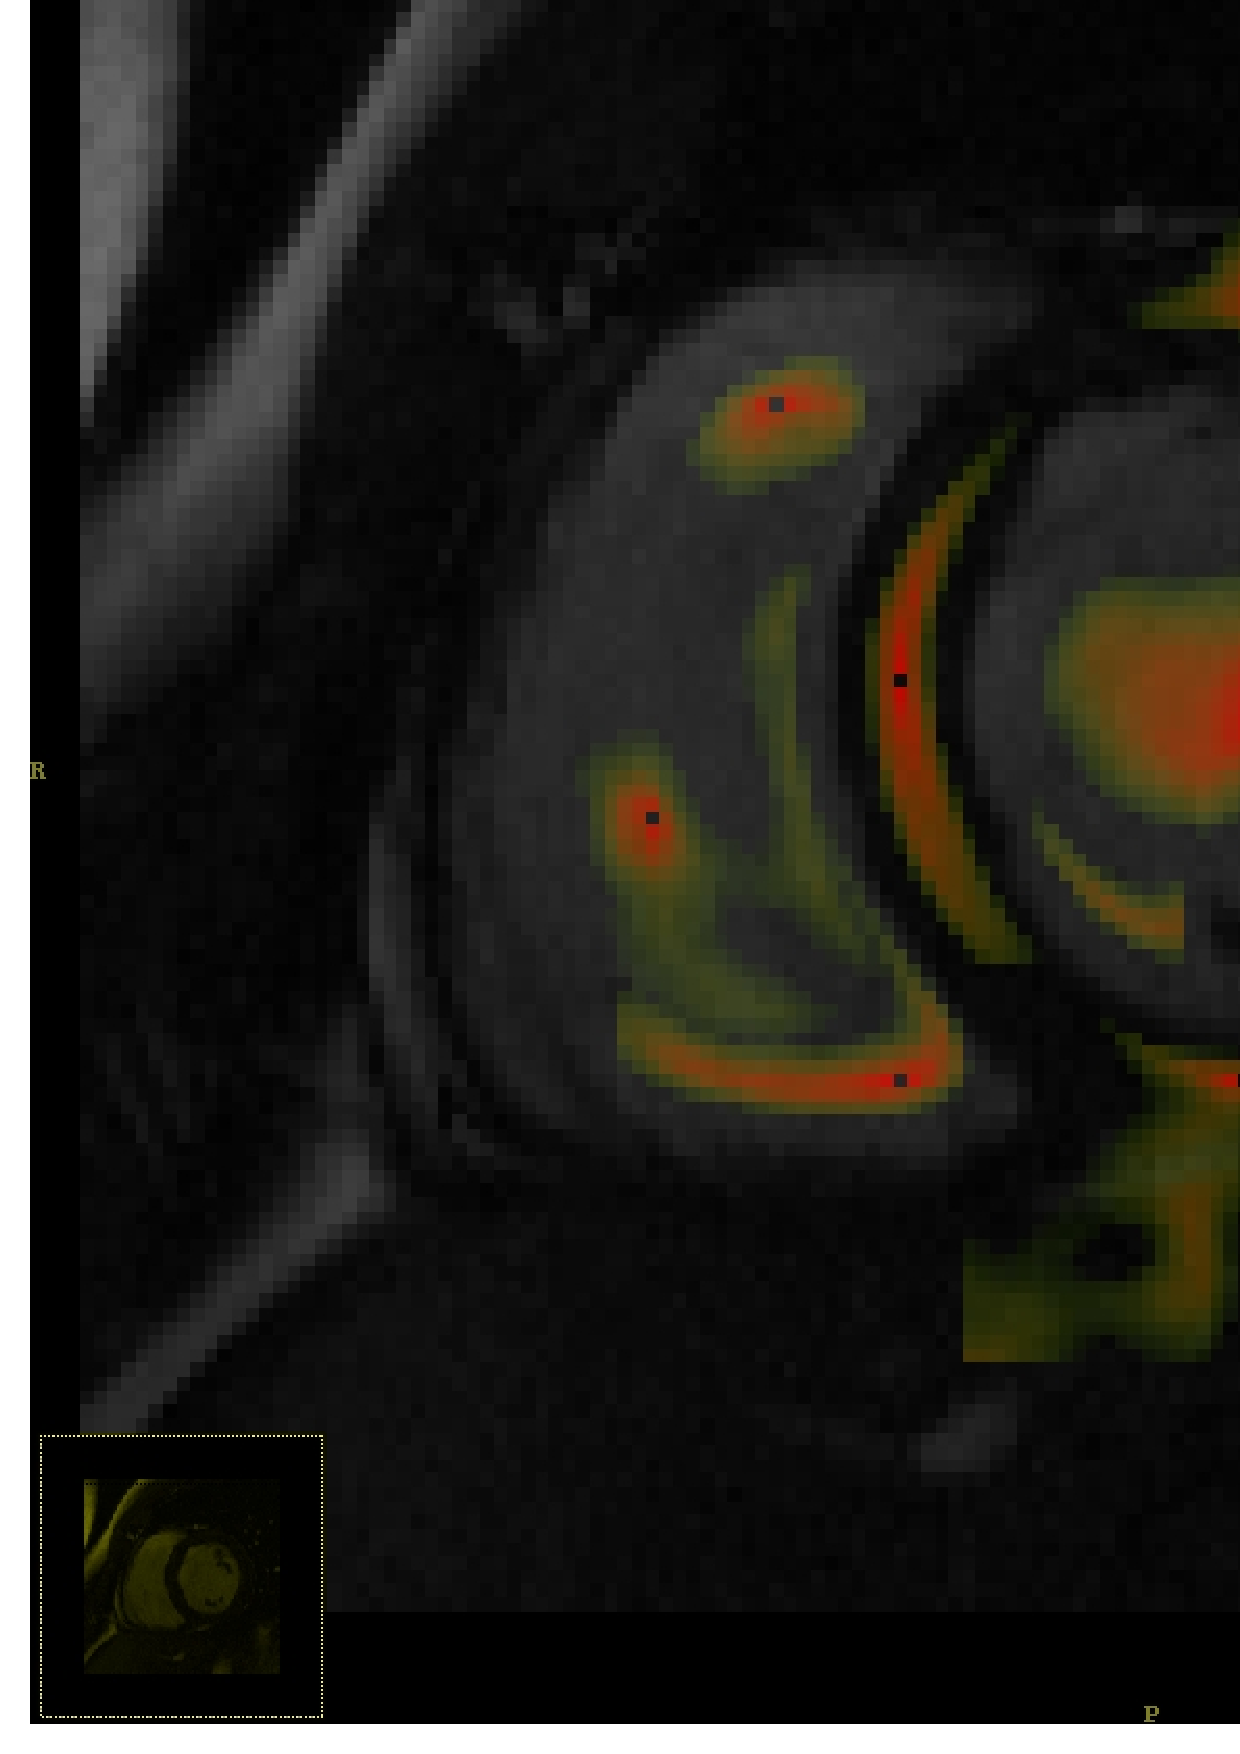
\includegraphics[scale=0.25]{images/wav_local.png} 
\caption{\em \small Wavelet-based attribute vector similarity. The matchmaps, or the similarity in the neighborhood of select points are shown.}
\label{wav-sim}
\end{center}  
\end{figure} 

The effectiveness of the wavelet attribute in capturing the uniqueness of a given voxel can be seen in Figure \ref{wav-sim}. We evaluate the similarity of the attribute vector with the voxels in its neighborhood. As can be seen the attribute vectors are able to localize the voxel effectively. The neighboring voxels show high similarity to the given voxel. The similarity drops as we move away from the voxel. Another thing to notice is that the similarity also drops as we cross over to the blood from the myocardium and vice-versa. Thus the wavelet attribute vectors effectively capture the local and global features of a given voxel. One problem with the wavelet attribute that can be seen in Figure \ref{wav-sim} is that we seem to get \textit{reflections} about blood-myocardium boundaries. This happens to a large part because the wavelet attributes calculated by \cite{wav} are rotation invariant. For cardiac motion estimation it is actually preferable not to have rotation invariant attributes. This will be done in the future.


\begin{figure}
\begin{center}
\subfigure[Original Frame on which the points were selected, with the points shown in blue.]{
\includegraphics[width=.30\textwidth]{images/frame-01}} 
\hspace{.15in}
\subfigure[The Target Frame, showing the original points in blue. The best correspondence is shown in yellow]{
\includegraphics[width=.30\textwidth]{images/frame-10}}
\caption{\em \small Wavelet-based attribute vectors for evaluating deformations within the same subject.}
\label{wav-twist}
\end{center}  
\end{figure}

%\begin{figure}
%\begin{center}
%\subfigure[Original Frame on which the points were selected, with the points shown in blue.]{
%\includegraphics[width=.30\textwidth]{images/wav-t1-06-03}} 
%\hspace{.1in}
%\subfigure[Slice - 1, on the Target Frame. As can be seen some points have moved out of the original plane. This happens because of twisting during the cardiac cycle.]{
%\includegraphics[width=.30\textwidth]{images/wav-t1-06-02}}
%\hspace{.1in}
%\subfigure[Original slice on the Target Frame, showing the matchmap and the original points in blue. The best correspondence is shown in yellow]{
%\includegraphics[width=.30\textwidth]{images/wav-t1-06-01}}
%\caption{Wavelet-based attribute vectors for evaluating deformations within the same subject.}
%\label{wav-twist}
%\end{center}  
%\end{figure} 

\subsection{Selecting the best correspondence point}

Instead of using inverse consistency for determining the best match for a given voxel as done in \cite{wav}, we instead use an alternate strategy. We compute the similarity $\varphi$ of the point $p$ defined on the end-diastole frame, $I_0$, to points within a search radius, $r$, in the image $I_t$. We test the similarity between the point $\bp$ on $I_0$ and the neighboring points, $\bp + \bepsilon$, on $I_t$, where $\|\bepsilon_i\| \le r$. The points in $I_t$ together with their similarity values to the point $\bp$ define a {\em matchmap} \cite{guest01}. This can be seen in Figure \ref{wav-sim}. We select the best corresponding point by integrating over the matchmap. We want to weight the points by the similarity, therefore we assign weights to the points based on their similarity,
\[
	\gamma_i = \varphi(\bW_{I_0}(\bp), \bW_{I_t}((\bp + \bepsilon_i)))
	%\gamma_i = \frac {\varphi(\bW_{I_0}(\bp), \bW_{I_t}((\bp + \bepsilon_i)))}{1 + |\bepsilon_i|^b},~~~~~~~~~b\ge2,
\]
where, $\bW_I(\bx)$ is the wavelet attribute vector at point $\bx$ on image $I$, and $\bp + \bepsilon_i$ is a point within the search radius.
%where, $W_I(\vec{x})$ is the wavelet attribute vector at point $\vec{x}$ on image $I$, and $\vec{\epsilon}_i$ is the perturbation applied to the point $\vec{p}$ within the search radius, and $b$ is a constant. 
%We use a value of 2.0 for $b$, so that points that are far away can still influence of the corresponding point if they match well. 
Using this, the best corresponding point, $\bx_c$, is given by the weighted mean of the points, where the weights are $\gamma_i$ defined above, 

\[
\bx_c = \frac {\sum \gamma_i (\bp + \bepsilon_i) } { \sum \gamma_i }
\]
the summation being evaluated over a neighborhood of the point $\bp$.

This makes the correspondence detection more robust and also imposes smoothness constraints. The results from this formulation can be seen in Figure \ref{wav-twist}. The best correspondence points are shown in yellow. These typically lie in another plane and are thus shown in two frames, one with the original points in blue and the other with the detected points. The twist within the myocardium is clearly visible. These results make us believe that along with smoothness constraints, the wavelet attributes along with the weighted correspondence estimation are best suited to extract cardiac motion fields.

We also observe that the wavelet attribute vectors are very effective in detecting correspondence across subjects. This can be seen in Figure \ref{fig:wav-sub}. Here the points in the template image are shown in blue. The detected corresponding points are shown in yellow. As we can see, the attribute vectors are able to identify the corresponding points both the in the end-diastole image, i.e., the one with no deformation and the end-systole image, the one with maximum deformation, Figure \ref{fig:wav-sub2}. Thus we see that the wavelet-based attribute vectors are both robust and accurate across time and across subjects. Also, the similarity computation between the attribute vectors, described in Section \ref{sec:attribSim} is very fast and thus makes the actual registration very efficient. 

\begin{figure}
     \centering
     \subfigure[The template image on which the points are selected. Shown here in blue.]{
          \includegraphics[width=.30\textwidth]{images/wav-p1-01-t1}
          \label{fig:wav-sub-tem}}     
     \hspace{.1in}     
     \subfigure[The subject image, same frame, adjacent slice. The best correspondence is shown in yellow.]{
          \includegraphics[width=.3\textwidth]{images/wav-p1-01-y}}
     %%\hspace{.05in}
     \hspace{.1in}
     \subfigure[The subject image, same frame, same slice. We show the selected points in the template space, overlaid in blue.]{
          \includegraphics[width=.3\textwidth]{images/wav-p1-01-b}}
     \caption{\em \small Attribute similarity across different Subjects}     
     \label{fig:wav-sub}
\end{figure}

\begin{figure}
     \centering
     \subfigure[The subject image shown further along cardiac cycle, slice - 3. One of the points is detected on this slice]{
          \includegraphics[width=.2\textwidth]{images/wav-p1-06-01}}
     %%\hspace{.05in}
     \hspace{.1in}
     \subfigure[The subject image shown further along cardiac cycle, slice - 2. One of the points is detected on this slice]{
          \includegraphics[width=.2\textwidth]{images/wav-p1-06-02}}
     %%\hspace{.05in}
     \hspace{.1in}
     \subfigure[The subject image shown further along cardiac cycle, slice - 1. Two of the points are detected on this slice]{
           \includegraphics[width=.2\textwidth]{images/wav-p1-06-03}}
     \hspace{.1in}      
     \subfigure[The subject image shown further along cardiac cycle, the same slice. The points picked in the template space are shown in blue.]{
           \includegraphics[width=.2\textwidth]{images/wav-p1-06-04}}
     \caption{\em \small Attribute similarity across different Subjects and different time frames}
     \label{fig:wav-sub2}
\end{figure}

\subsection {Distinctiveness of attribute vectors}
\label{sec:wav-distinctive}
In order to be able to pick focus points to drive the registration, we need to be able to select attribute vectors based on how distinctive they are. Doing this will allow us to robustly perform the registration in a fast hierarchical manner. This also allows us to select focus points automatically based on the distinctiveness of the attribute vectors. Also we weight the similarity of the points, during the energy function evaluation by the distinctiveness of the point. If we perturb each point in the end-diastole image $I_0$ and evaluate the best correspondence point for each of these points, we will get a scatter of best correspondence points. The distribution of this scatter of points provides information about the robustness of each match to image $I_t$ \cite{guest01}. 

\begin{figure}
\begin{center}
\includegraphics[scale=0.25]{images/dist_explain.png} 
\caption{\em \small Different kinds of matchmaps. Points A are points with high distinctiveness as their spread is small. Point B has low distinctiveness as it has a large spread. Points C also have relatively low distinctiveness, since the spread is large along one of the axes}
\label{dist-exp}
\end{center}  
\end{figure}

To understand how we define the distinctiveness of a given voxel based on the wavelet attributes, consider Figure \ref{dist-exp}. We can see that different voxels produce different scatters based on the local and global characteristics of the underlying image. Although we get sharp peaks for all three types, (A,B, and C), we observe that for {\bf A} the scatter is localized and the spread is uniform and small in all directions. In case of {\bf B}, the spread is more or less uniform but it is large. The distinctiveness of such points is low, because there are a lot of points which are relatively far from the actual point that have sufficiently high similarity. The confidence in the similarity of such points is lower since we could be sufficiently far from the best point (in mm) and still have a fairly high similarity. Such points can increase the error in registration, and should therefore be avoided. The third set of points, {\bf C} is also not very distinct, because although they are heavily localized in one direction, there is a very large spread along the principal axes. Again such points can increase the error in registration and should be assigned low {\em distinctiveness}. 

\begin{figure}
\centering
     \subfigure[Distinct point that has low spatial spread and is static, i.e., has no motion]{
          \includegraphics[height=.27\textwidth]{images/dist-a}
          \label{fig:dist-a}
          }
     \hspace{.1in}     
     %%\hspace{.05in}
     \subfigure[Distinct point, that has low spatial spread and has temporally smooth motion]{
          \includegraphics[width=.27\textwidth]{images/dist-b}
          \label{fig:dist-b}
          }
     \hspace{.1in}     
     \subfigure[Non distinct point that has large spatial spread and haphazard temporal motion]{
          \includegraphics[width=.27\textwidth]{images/dist-c}
          \label{fig:dist-c}     
          }
     \caption{Distinctiveness of a point over a sequence}     
     \label{fig:dist-seq}
\end{figure} 

The situation is a bit different when we consider a sequence of such images, and their matchmaps over time. Some of the common cases that can occur are shown in Figure \ref{fig:dist-seq}. One common case is of points that are localized spatially and temporally consistent, as shown in Figure \ref{fig:dist-a}. These kinds of points typically can be found outside the pericardium, i.e., tissues and bones which do not move much during the cardiac cycle. Figure \ref{fig:dist-b} shows the case that is ideally preferred for points within the myocardium. These are points whose spatial spread is low, and temporally smooth motion can be observed. Figure \ref{fig:dist-c} shows the case of a point whose matchmaps are scattered across slices, and the confidence in estimating the location of this point across slices is low. Therefore, we assign a low distinctiveness to such points. This amounts to a distinctive point having a large spread along the time axis, and much smaller localized spreads along the spatial dimensions.

We extend this to the 4D case, where the only difference is that we wish for the spread along the time axis to be large, and the other three to be small. In order to compute the distinctiveness of the selected point, we calculate the eigenvalues and eigenvectors from the moment of inertia matrix obtained from the 4D matchmap. The 4D moment of inertia matrix of the matchmap is defined as,

\begin{equation}
\label{eq:moi}
I = \sum_i \gamma_i \left[ 
\begin{array}{cccc}
	y_i^2+z_i^2+t_i^2 & -x_iy_i & -x_iz_i & -x_it_i \\
	-x_iy_i & x_i^2+z_i^2+t_i^2 &  -y_iz_i & -y_it_i \\
	-x_iz_i & -y_iz_i & x_i^2+y_i^2+t_i^2 &  -z_it_i \\
	-x_it_i & -y_it_i  &  -z_it_i & x_i^2+y_i^2+z_i^2 
\end{array}
\right]
\end{equation}

We prefer points whose similarity matchmaps are spatially localized and compact. They should also be temporally smooth. This means that the 4D scatter in a 4D neighborhood for distinct points should be a 4D cylinder. We therefore compute the eigenvalues of the moment of inertia matrix, defined in (\ref{eq:moi}), and assign high distinctiveness to all points which have one large eigenvalue and three small eigenvalues. Here we are basically trying to keep the spatial spread low. Because of the way the 4D matchmap is evaluated, the temporal spread will be large. For points which do not move much, the principal eigenvector will be aligned with the {\em time} axis. Correspondingly as the motion of the point in question increases, the angle between the principal eigenvector and the {\em time} axis will increase. Since we wish to give more importance to points with large motion. Therefore we scale the distinctiveness factor by the angle between the principal eigenvector and the {\em time} axis.

%In the 3D case, there are three eigenvalues and eigenvectors. If all the eigenvalues are small, the tentative corresponding points are clustered near a point. If the second and third eigenvalues are small, the tentative corresponding points are scattered along a line; and if only the third eigenvalue is small, they are scattered in a plane. When all the eigenvalues are large, the tentative corresponding points are widely scattered. We use the values of these eigenvalues as an estimate of how reliable a given point is for determining correspondence. When the points are widely scattered, i.e., the case when all three eigenvalues are large, we place low confidence on the reliability of that point. Conversely, the best points are those which are clustered about a point, i.e., those that have all small eigenvalues. 

\begin{figure}
	\centering
	  \subfigure[Distinctiveness calculated over the whole image. We can see that it is low along the peripheries and also within the blood pool.]{\includegraphics[height=.25\textheight]{images/hari-dist2}}
	  \hspace{.15in}
		\subfigure[Overlay of the distinctiveness to show the distinctiveness on the myocardial region]{\includegraphics[height=.25\textheight]{images/distinctiveness}}
	\caption{The distinctiveness of voxels, based on the wavelet attribute vectors}
	\label{fig:distinctiveness}
\end{figure}

The distinctiveness of the voxels as computed by this method is shown in Figure \ref{fig:distinctiveness}. As can be seen this is proportional to both the level of structural as well as motion relation features, which is what we are trying to extract. We can use this these {\em distinctiveness} values to compute a multiresolution set of {\em focus} points. 


\section{Estimating the Cardiac Motion Field}
\label{sec:CarMot}

Cardiac motion estimation is the problem of determining a transformation that captures the motion of every point in the myocardium over the cardiac cycle. If we can register 3D images acquired at different phases of the cardiac cycle to each other, then we have an estimate of cardiac motion. Thus we can formulate the problem as one of being able to track (detect correspondence) of a small set of points on the myocardium over the entire cardiac cycle. 

These points are the ones whose motion can be estimated most reliably. These are selected based on their distinctiveness, Section \ref{sec:wav-distinctive}. This makes the registration more robust as it is not affected by points with low distinctiveness, i.e., those points whose correspondence cannot be determined with high confidence. Another advantage of using the {\em focus} points is that it makes the similarity computation faster. It also reduces the dimensionality of the cost function, making the optimization more robust and faster. All these factors together make the current formulation robust and fast. 
%We solve only for the correspondence of a small set of {\em focus} points because we want the estimation process to be fast. 
Since the myocardium moves as one connected object and the motion is smooth, we can interpolate the transformation at the focus points to get the transformation over the whole myocardium. 

The problem of motion estimation from cardiac cine images is ill posed, and relying solely on image similarity, even with very accurate similarity measures is not sufficient to capture the true motion of the heart. Current cardiac motion estimation methods rely on image similarity measure to drive the motion estimation, and typically incorporate a regularizer to smooth the deformation field. We propose to instead maximize the similarity between the wavelet attributes, subject to the motion estimate constrained by a mechanical model of the heart, which has been discussed in Section \ref{sec:model}.

The result of a 4D scan of a beating heart is a periodic sequence of $N$ 3-$D$ images,
\[
I(\bx,t) = \{I_t(\bx), 0\le t < N\}
\] 
where $I_0$ is the end-diastolic image. We define the motion field as the transformation $\bchi ( \bx, t )$ defined over the image space. The transformation maps a point $\bx$ in the end-diastole frame $I_0$ of the image to its corresponding point in frame $I_t$ at time $t$. This is illustrated in Figure \ref{fig:motion}. The displacement field $\bU( \bx, t )$  defines the mapping from the coordinate system of the end-diastole image $I_0$ to the image at time $t$, $I_t$. The transformation and the displacement are related as, $\bchi( \bx ,t ) = \bx + \bU( \bx, t)$.

\begin{figure}
\begin{center}
\includegraphics[width=.75\textwidth]{images/motion-est} 
\caption{Formulation of the cardiac motion extraction problem.}
\label{fig:motion}
\end{center}  
\end{figure} 

A sparse set of focus points $\bp \in \Omega$ needs to be defined on the end-diastole image $I_0$. This can either be done manually, by the user, or using some feature extraction policy. Automatic focus point selection as described in Section \ref{sec:wav-distinctive} is used to select focus points at different resolutions to be used with the multiresolution approach. These points are tracked through the entire sequence $I(\bx, t)$ in order to determine the correspondences and estimate the motion field $\bchi ( \bx, t )$. We solve an energy minimization problem where we solve for the deformation vectors at each of these points at each time frame.

To allow the registration algorithm to focus on different sets of points adaptively during different stages of image registration, each point should have it's own energy term and the overall energy function should be a weighted summation of energy terms of all the points. Therefore, by hierarchically assigning weights, $\eta ( \bx)$,  according to the distinctiveness of the attribute vectors (Section \ref{sec:wav-distinctive}), we can focus on the most suitable points to actively drive the image registration. This increases the reliability of the motion estimation as it is not affected by the similarity estimates of unreliable points. The other benefit is that of improved speed of the motion estimation. If we were to solve for the displacement at every grid point on the image, then the dimensionality of the cost function that we are minimizing will be extremely high. Also the cost function evaluation would be much more expensive. Solving for the displacements at only the focus points, allows us to reduce the dimensionality of the problem and also makes the cost function evaluation much faster. Thus the procedure approximates a very high-dimensional cost function (equal to the number of points in the image sequence) by a significantly lower-dimensional cost function of only the active points. This makes the minimization process much faster and also less susceptible to getting trapped in local minima, as it is a function of the focus points for which we can find relatively unambiguous matches. The method also performs much better than a simple subsampling of the original grid to reduce dimensionality, since in essence we create an adaptive grid that is dense in areas with more distinctive features and sparse in areas which are relatively static or where the confidence in the similarity is low.

We present the motion problem as a non-linear pde constrained optimization problem. Most systems can be thought of as having certain control parameters $g$, which directly or indirectly affect the process' state $\phi$. An optimization problem can be thought of as one of finding controls $g$ and states $\phi$ such that a cost functional $\mathcal{C}(\phi, g)$ is minimized subject to $\mathcal{F}(\phi, g)=0$.  Here the cost functional $\mathcal{C}(\phi, g)$ is a measure of the how close the current state is to the desired one. $\mathcal{F}(\phi, g)=0$ is a constraint on the relationship between the states and the controls. For the problem of cardiac motion estimation, we solve for the forces $\tau$ in the myocardial fibers and obtain the states $\bu$, the displacements produced as a result of these forces. The constraint, $\mathcal{F}(\bu, \tau)=0$ is the mechanical model described in Section \ref{sec:model},

\[
\mathcal{F}(\bu, \tau) = \rho_0\dudtsq - \mbox{Div}(\lambda \ln\mathcal{J}\bF^{-T} + \mu(\bF -\bF^{-T})) - \sigma\bF\bn = 0 \mbox{~~~~in~} \Omega
\]

The cost functional that we minimize, is the wavelet similarity term discussed earlier in Section \ref{sec:attribSim}. The similarity is computed between the wavelet attribute vectors at the point $\bchi ( \bx, t )$, $\bW ( \bchi ( \bx, t ) )$ and at the point $\bchi ( \bx, t + 1 )$, $\bW ( \bchi ( \bx, t + 1 ) )$. The Energy function for point similarity, summed over all the focus points, $\bp$, over all time frames is,
\begin{equation} 
\label{eq:wav-sim}
   \mathcal{C}(\bu, \tau) = \sum_{t = 0}^{N - 1} \sum_{\bx \in \{\bp \}} \eta (
     \bx) \left( \sum_{\bz \in n ( \bx, 0 )} \varphi \left(
     \bW ( \bchi ( \bz, t ) ), \bW ( \bchi ( \bz, t + 1 ) ) \right)
     \right) 
\end{equation}

The importance of each point $\bx$, in the registration is determined by the corresponding parameter $\eta (\bx )$, which is designed to be proportional to the distinctiveness of the point's wavelet-based attribute vector. The match for each point $(\bx, t)$ is evaluated in it's 3-$D$ neighborhood $n ( \bx, 0 )$, by integrating the similarity measure between the attribute vector $\bW( \bchi ( \bz, t ) )$  of every neighboring point $( \bz, t )$ and the attribute vector $\bW ( \bchi ( \bz, t+1 ) )$ of the corresponding point in the adjacent time frame of the sequence. The is equivalent to matching image patches or volumes between the two images because of the following two reasons,

\begin{itemize}
	\item The attribute vector is calculated in a local neighborhood and therefore represents information in the neighborhood of the voxel in question.
	\item We sum over the similarities in the neighborhood of $\bx$ when evaluating the wavelet similarity term (\ref{eq:wav-sim}).
\end{itemize}

The size of the neighborhood is large initially and decreases gradually with the progress of the deformation, thereby increasing robustness and accuracy of the motion estimation. As the neighborhood size is decreased we also change the weights for the multi-resolution attribute vectors similarity, increasing the weights for the fine features and decreasing the weights on the global features. This is equivalent to reducing the size of the image patches being matched as we move to the higher resolutions.

The optimization algorithm can be solved by using the following algorithm,

%\begin{algorithm}
%\caption{Cardiac Motion Estimation Algorithm} \label{MotAlg}
%\begin{algorithmic} [1]
%\STATE i=0, Initial guess for forces, $\tau^{(0)}$
%\WHILE {solution not converged}
%\STATE \textbf{solve} $\mathcal{F}(\bu^{(i)}, \tau^{(i)})=0$ to obtain displacements; \COMMENT{The mechanical model}
%	\STATE \textbf{compute} the gradient of the functional $\frac{\partial \mathcal{C}}{\partial \tau}(\bu^{(i)}, \tau^{(i)})$;
%	\STATE \textbf{compute} the step $\delta \tau^{(i)}$
%	\STATE \textbf{set} $\tau^{(i+1)} = \tau^{(i)} + \delta \tau^{(i)}$
%\ENDWHILE
%\end{algorithmic}
%\end{algorithm}


\section {Periodicity Constraint}
Since the image sequence is periodic, i.e.,  the first image $I_0$ and the last image $I_{N-1}$ are also temporal neighbors, as shown in Figure \ref{fig:motion}. We impose a hard constraint on the deformations to return a point $\bx$ to itself after the full cardiac cycle, i.e., $( \bx, 0 ) = \chi ( \bx, N-1 )$. This is done by ensuring that during each step of the minimization,

\begin{equation}
\sum_{\bx \in \{ \bp \}} \| \bchi ( \bx, N-1 ) - ( \bx, 0 ) \| = 0 
\end{equation}

%\subsection {Interpolation of the deformation field}
%\label{sec:interpolation}

%Since we only solve for the motion field at the sparse set of points $\bp$, we need to interpolate to get the transformation over the whole image space. In order to do this, we obtain a 3D Delaunay tetrahedralization \cite {delaunay34}\cite{meshkat91} of the set of focus points $\bp$. We then interpolate for the value of the deformation field at points inside the tetrahedron using cubic interpolation employing barycentric coordinates.

%\subsection{The multi resolution framework}
%\label{sec:multires}

%The multi-resolution approach makes the system more robust and helps the system avoid getting struck in local minima. We perform the motion estimation at three different resolutions. We start with a sparse set of points defined on the template space. The similarity is evaluated on a large neighborhood and the attribute vectors are weighted heavily in favor of the low resolution attributes. Once the low resolution estimate converges, we increase the number of focus points. The focus points are added adaptively to the tetrahedra that have maximum volumetric change. We don't need to recompute the entire mesh because the delaunay tetrahedralization is incremental in nature. At the middle-resolution, we also reduce the neighborhood over which the attribute similarity is evaluated and the weights of the attribute vectors are balanced between the three levels. At the high-resolution estimation stage, we add more focus points adaptively and also change the weights of the attribute vectors to favor the high-resolution attributes. Thus the whole framework works in a multi-resolution way to best estimate the cardiac motion field.

%\subsection{Energy Minimization}
%\label{sec:emin}

%We need to choose an appropriate solver which will provide a practically feasible solution. Since we need to optimize in extremely high dimensions with non-linear cost functions and non-linear constraints, it is extremely important that select the appropriate optimization package that can perform fastest and also guarantee global convergence. We use \verb|IPOPT| \cite{Wachter04a}, a nonlinear programming solver employing the primal-dual interior point method in conjunction with filter methods that ensure global convergence. Global convergence implies that our solution will reach a local optima irrespective of the starting point supplied, although the convergence may be dependent on the starting point. 

%Our preference towards \verb|IPOPT| was motivated by the scalability of the interior point approach \cite{Nocedal99a} over other approaches that make use of active set strategies which do not scale well for large number of inequality, in our case, bound constraints. The gradient of the objective function is computed using a higher order finite differencing scheme \cite{Dennis83a}. When we test for smaller problem sizes, we make use of a second order finite differencing scheme for the Hessian, whereas for larger problem sizes we use the optional quasi-Newton updating of the Hessian. For any solver, it is important to choose an appropriate stopping criterion, we choose the error of constraint violation. Let $||E||$ be the norm of the error violation of the optimality conditions. We stop when $||E|| = ||E||_{0} \times 10^{-8}$ where  $||E||_{0}$ is the error at the initial iterate.
	     
\section{4D Cardiac Registration}
\label{sec:4dreg}

In order to be able to perform group analysis on a set of 4-$D$ scans of the beating heart to statistically characterize structural and functional qualities of the heart, we need to be able to perform a 4-$D$ registration between an atlas of a normal heart, the template $T$, and the subject $S$. Here 4-$D$ refers to the 4-dimensional space in which the beating heart resides, namely the regular 3-$D$ eucledean space and the 1-$D$ time space. The 4-$D$ registration will enable to to quantify the differences between a normal and an abnormal heart. Our goal is to estimate a 4-$D$ transformation that maps a given point $(\bx, t)$ in the subject to a point in the template. This transformation characterizes both the structural as well as the functional (myocardial wall motion) differences between the subject and the template. The 4-$D$ registration builds on the cardiac motion estimation algorithm described in Section \ref{sec:carMot}. The problem formulation is summarized in Figure \ref{fig:reg4d}. It is only in recent years that imaging modality acquisition technology has developed to an extent to allow us to acquire 4-$D$ datasets. These are still the early days and currently available 4-$D$ datasets are plagued by a number of problems. The three most common modalities which are used to acquire 4-$D$ datasets are MR, Ultrasound and CT. Each of these modalities have their advantages and associated problems. 
%We summarize the advantages and disadvantages of each of these in Table \ref{tab:4dmod}. These are specifically evaluated with cardiac imaging applications in mind. 
Since these modalities are so different, it is important while designing a 4-$D$ registration algorithm to keep in mind the the advantages and shortcomings of the underlying imaging modality. The features being used for correspondence detection, the energy function being minimized and the set of constraints imposed need to be carefully selected keeping the strengths of the modality in mind. Specifically, for the case of 4-$D$ image registration for cardiac applications, MR Cine sequences have been popular \cite{perperidis04}. Detecting correspondences across different patients in MR Cine sequences is not an easy task, especially for cardiac datasets, which are poor in features both because of the inherent geometry of the heart and because of shortcomings in the acquisition. 

One of the key problems when dealing with 4D MR cine sequences is that inter-slice spacing and the slice thickness are quite large. This implies that anatomical structures (features) that are imaged under one patient might not be present in the other patient's scan. This is illustrated in Figure \ref{fig:slice-thick}. This is the reason that the wavelet based attribute vectors, which evaluate the similarity in a neighborhood around the point perform much better than other local measures of similarity. 

%In the 4-$D$ case, we have additional inputs to help in correspondence detection across subject. This is the knowledge of the motion fields of the subject and the template, which have been estimated as described in Section \ref{sec:carMot}. This helps because, as the heart moves, parts of the heart that were not images earlier because of the large slice thickness, now get imaged. Therefore, by adding a constraint to keep the motion fields of the template and the subject we improve the accuracy of the correspondence detection and thereby the estimation of the 4-$D$ transform. It is also important to impose constraints that give importance to temporal consistency along with temporal smoothness. This is something that is not addressed by work already done in this field \cite{perperidis04}. We shall elaborate on these constraints later in the section.

In the 4-$D$ case, we have additional information that helps us in correspondence detection across subjects. This is the knowledge of the motion fields of the subject and the template, which can be estimated {\em a priori} as described in Section \ref{sec:carMot}. It is important to realize that if better estimates of myocardial motion are available by other means, such as tagged images or MR phase contrast imaging, they can be used directly instead of estimating the motion from the MR Cine sequences. We use the motion field to ensure that the correspondence detected between the template and the subject is consistent during the entire cardiac cycle. Apart from ensuring a temporally smooth and consistent transformation, this also helps in better correspondence detection. As the heart moves, parts of the heart that were not imaged earlier because of the large slice thickness, now get imaged. Therefore, by adding a constraint to keep the motion fields of the template and the subject consistent, we improve the accuracy of the correspondence detection and thereby the estimation of the 4-$D$ transform. It is also important to impose constraints that give importance to temporal consistency along with temporal smoothness. This is something that is not addressed by work already done in this field \cite{perperidis04}. We shall elaborate on these constraints later in the section.

\begin{figure}
\centering
     \subfigure[Points {\bf b} and {\bf d} get imaged, whereas points {\bf a} and {\bf c} do not get imaged.]{
          \includegraphics[width=.4\textwidth]{images/slice-thick-a}
          \label{fig:thick-a}
          }
          \hspace{.15in}
     %%\hspace{.05in}
     \subfigure[Because of cardiac motion, at a different part of the cardiac cycle, points {\bf a} and {\bf c} get imaged. However, at this time {\bf b} and {\bf d} are no longer imaged.]{
          \includegraphics[width=.4\textwidth]{images/slice-thick-b}
          \label{fig:thick-b}
          }
     \caption{Imaging problems due to large inter-slice spacing}     
     \label{fig:slice-thick}
\end{figure} 

We first perform an affine registration to normalize the subject. This is essential to make the 4-$D$ transformation and consequently the classification independent of variations in sex, age, weight and height of the patient. Also the datasets might vary because of differences in the image acquisition procedure. Therefore it is extremely important to perform spatio-temporal normalization of the datasets before performing the 4-$D$ registration.

\subsection{Spatio-Temporal Affine Registration}

When registering two 4-$D$ image sequences, spatial alignment of the corresponding frames in not sufficient as the frames could correspond to different phases in the cardiac cycle of the heart. This difference arises due to,
\begin{itemize}
	\item Difference in acquisition parameters like initial offset in the acquisition of the first frame and different frequency in the acquisition of subsequent frames. 
	\item Difference in the length of the cardiac cycle, which arise due to different patients having different heart rates.
	\item Difference in the dynamic properties of the heart, i.e., differences in lengths of systole and diastole.
\end{itemize}

The spatial component of the affine transform comes due to the following differences,
\begin{itemize}
	\item Different heart sizes and orientation because of variations in sex, age, height and weight of the patient.
%	\item Difference in acquisition parameters like pixel spacing and slice thickness.
	\item Variations in the way the patient is placed inside the scanner.
\end{itemize}

Spatio-temporal alignment will enable comparison between corresponding anatomical positions and corresponding phases in the cardiac cycle of the hearts. Perperidis et al suggest a possible normalization method \cite{perperidis04} by extending their B-Spline based registration algorithm as a combination of a 3-$D$ spatial registration and a 1-$D$ temporal registration. They decouple the 4-$D$ mapping into independent spatial and temporal components. 

%\begin{table}
%	\begin{center}
%		\begin{tabular}{|c|c|c|}
%		\hline
%			Modality & Advantages & Disadvantages \\
%			\hline
%			MR & High Temporal Resolution & Low inter-slice spacing \\
%			US & Easy to acquire & Poor image information \\
%			CT & High spatial resolution (sub mm) & Poor temporal resolution \\
%			\hline
%		\end{tabular}
%	\end{center}
%
%	\caption{Comparison of current 4-$D$ modalities}
%	\label{tab:4dmod}
%\end{table}

We use a similar framework during the initial affine registration part of our 4-$D$ registration. However although it is reasonable to assume that the temporal and spatial transformations are independent, they do affect each other while estimating one with an approximate solution of the other. We do not assume that the two are independent and solve iteratively to get the optimal affine transformation. Since we are performing affine registration, it is better to use a metric that is evaluated over the entire image space. Normalized mutual information \cite{stud99} has been shown to perform well in similar registration problems. We use NMI as the similarity measure, which is given by:
\begin{equation}
NMI(A, B) = \frac{H(A) + H(B)}{H(A,B)}
\end{equation}
here $H(A)$ and $H(B)$ denote the separate entropy values of images $A$ and $B$, respectively. $H(A,B)$ is the joint entropy, i.e., the entropy of the joint probability distribution of the image intensities. We use the Shannon measure of entropy, $-\sum_{p\in P}p\log p$ for a probability distribution $P$.

First we estimate the 3D affine transformation $\mathcal{A}(\bx)$ by performing a 3D affine registration between the two end-diastole images. This is done by maximizing the normalized mutual information metric described above. We can present this as an energy minimization problem by minimizing the negative of the normalized mutual information. That is the energy that is minimized is defined as
\begin{equation}
E = -NMI(T_0(\bx), S_0(\mathcal{A}(\bx)) = -\frac{H(T_0(\bx)) + H(S_0(\mathcal{A}(\bx)))}{H(T_0(\bx),S_0(\mathcal{A}(\bx)))}
\end{equation}
where $T_0$ and $S_0$ are the end-diastole frames of the template and the subject sequences respectively.

Once this is estimated we then estimate the temporal shift and scale of the subject with respect to the template, using the estimated spatial transformation. The temporal normalization aligns the two sequences and makes the subject $S$ have the same number of frames $N$ as the template $T$. We follow this with a second set of spatial registration. The difference in this case is that the similarity is evaluated over all image pairs in the sequence. The energy function that is minimized during this step is,
\begin{equation}
E = -\sum_{i=0}^{N-1}NMI(T_i(\bx), S_i(\mathcal{A}(\bx)))=-\sum_{i=0}^{N-1}\frac{H(T_i(\bx)) + H(S_i(\mathcal{A}(\bx)))}{H(T_i(\bx),S_i(\mathcal{A}(\bx)))}
\end{equation}

Since the temporal normalization has been performed, the image pairs correspond to each other. We iterate over the last two steps till they converge and we have the final 4D affine transformation.

The results of the affine registration are shown in Figure \ref{fig:affine4d}.

\begin{figure}
     \centering
     \subfigure[The Template Image]{
          \label{fig:t1}
          \includegraphics[width=.4\textwidth]{images/t1}}
     %%\hspace{.05in}
     \subfigure[The Subject Image]{
          \label{fig:p1}
          \includegraphics[width=.4\textwidth]{images/p1}} \\
     %%\hspace{.05in}
     \subfigure[The Subject warped to the template space]{
           \label{fig:affine}
           \includegraphics[width=.4\textwidth]{images/affine}}
     \caption{The result of applying the 4-D affine transform to the subject image}
     \label{fig:affine4d}
\end{figure}

%% Results of the affine registration.

In the following steps it is assumed that the subject $S$ has been warped to the template space using the results of the affine registration. Both the sequences have $N$ frames each at the end of the affine registration.

\subsection{Attribute Vector}

We use the same wavelet-attribute vector as described in Section \ref{sec:wav}. As was shown in Section \ref{sec:wav}, the wavelet attribute vectors robustly and effectively detect correspondence across patients even with deformations present. The wavelet attribute at location $( \bx, t )$ is represented as  $\bW( \bx, t )$. 

\begin{figure}
\begin{center}
\includegraphics[width=.9\textwidth]{images/4dreg} 
\caption{Formulation of the 4D registration problem}
\label{fig:reg4d}
\end{center}
\end{figure} 

\subsection{Combined motion field extraction and 4D registration}

We now describe the algorithm for 4D registration. Since we are trying to quantify the difference between the subject $S(\bx, t)$ and the template $T(\bx, t)$, we need to compute the 4-$D$ transformation that transforms the subject to the template space. Both are 4D image sequences and the intensity at any location  $( \bx, t )$ can be accessed by, $T ( \bx, t)$ and $S ( \bx, t )$. The attribute vector $\bW$ at a given location $( \bx, t )$  is represented as $\bW_T(\bx, t)$ for the template and $\bW_S(\bx, t)$ for the subject.

We also define the following transformations:
\begin{itemize}
  \item $\bchi_T ( \bx, t )$: The motion field defined over the template
  space. The transformation maps a point $\bx$ in the end-diastole frame
  of the template to its corresponding point in frame at time $t$.
  
  \item $\bchi_S ( \bx, t )$: The motion field defined over the subject space.
  The transformation maps a point $\bx$ in the end-diastole frame of the
  subject to its corresponding point in frame at time $t$.
  
  \item $H_{T \leftarrow S} ( \bx, t )$: The 4d transformation that maps a
  4-$D$ point $( \bx, t )$ from the subject to the template space. We shall use $H ( \bx, t )$ to imply this transformation by default. The inverse transformation, $H_{S \leftarrow T} ( \bx, t )$ will be written as $H^{-1} ( \bx, t )$.
\end{itemize}
These transformations along with the formulation of the 4-$D$ registration problem are illustrated in Figure \ref {fig:reg4d}. We first compute the template motion field and the subject motion field. We then compute the 4-$D$ transformation using the two motion fields as additional constraints that help us better estimate the 4-$D$ transformation.

\subsection{Estimating the Template and Subject Motion Field}

We compute the template motion using the algorithm described in the previous section \ref{sec:CarMot}. If better estimates for the motion fields of either the subject or the template are available, say from tagged MR images or other methods, these can be used directly rather than estimating it using the method described. Depending on how much time is available for the the 4D registration, we have two strategies. The faster method is to compute the robust focus points based purely on the template image. This is done offline and needs to be done once and is therefore faster. The better albeit slower method is to compute the focus points by computing the focus points using the template and the subject, as described in Section \ref{sec:wav-distinctive}. This will need to be computed for each subject individually. A qualitative assessment will have to be done in the performance improvement in the registration as a result of using subject specific distinctiveness calculation.

\subsection{Estimation of 4D deformation field }

The problem is again posed as one of minimizing an energy function. We estimate the 4D deformation field that best maps the subject to the template and is also consistent with the template motion field $\bchi_T ( \bx, t )$ and the subject motion field $\bchi_S ( \bx, t )$. These three transformations are not independent and the two motion fields impose a strong constraint on the 4-$D$ deformation field. This relation can be expressed as:

\begin{equation}
\label{eq:4d-mot-rel}
\bchi_S ( \bx, t ) = H^{-1} ( \bchi_T ( H (\bx, 0 ), t ) )
\end{equation}

We define an energy function that incorporates the similarity between the template and the warped subject image. There is an additional energy term that is added to make the 4-$D$ transformation consistent with the two motion fields. The energy function also incorporates terms for smoothness of the deformation. The energy function that our 4D registration algorithm minimizes is defined as follows:
\begin{equation}
	E = E_F + E_B + E_C + E_{Smooth}
\end{equation}
We shall now define each of these terms in detail and the role they play in the proper estimation of the 4-$D$ transformation.

\subsubsection{Similarity}
In order to make the registration independent of which of the two sequences are treated as the template, the energy function should be symmetric to the two sequences being registered. Therefore we evaluate both the forward transformation $H^{-1} ( \bx, t )$ and the backward transformation $H ( \bx, t )$ and force them to be consistent with each other. These two evaluations give rise to the forward and backward energy terms, $E_F$ and $E_B$, respectively. These terms are defined as:
\begin{eqnarray}
  E_F &=& \sum_{t = 0}^{N - 1} \sum_{\bx \in \Omega_T }
  \eta_T ( \bx, t ) \left( \sum_{( \bz, \tau ) \in n ( \bx, t
  )} \varphi \left( \bW_T ( \bz, \tau ), \bW_S ( H^{-1} ( \bz, \tau
  ) ) \right) \right) \\
  E_B &=& \sum_{t = 0}^{N - 1} \sum_{\bx \in \Omega_S }
   \eta_S ( \bx, t ) \left( \sum_{( \bz, \tau ) \in n ( \bx,
   t )} \varphi \left( \bW_T ( H ( \bz, \tau ) ), \bW_S ( \bz,
   \tau ) \right) \right)  
\end{eqnarray}
   
The importance of each point $(\bx, t)$, in the forward energy term is determined by the corresponding parameter $\eta_T (\bx, t )$, which is designed to be proportional to the distinctiveness of the point's wavelet attribute vector $\bW_T ( \bx, t )$ on the template. Similarly the importance of each point $(\bx, t)$, in the backward energy term is determined by the corresponding parameter $\eta_S (\bx, t )$, which is designed to be proportional to the distinctiveness of the point's wavelet attribute vector $\bW_S ( \bx, t )$ on the subject. The match for each point $(\bx, t)$ is evaluated in it's 4-$D$ neighborhood $n ( \bx, t )$, by integrating the similarity measure between the attribute vector $\bW_T ( \bz, \tau )$  of every neighboring point $( \bz, \tau )$ and the attribute vector $\bW_S ( H^{-1} ( \bz, \tau ) )$  of the corresponding point in the subject. The same is true for the backward energy term. The size of the neighborhood is large initially and decreases gradually with the progress of the deformation, thereby increasing robustness and accuracy of the motion estimation. As the neighborhood size is decreased we also change the weights for the multi-resolution attribute vector's similarity, increasing the weights for the local features and decreasing the weights on the global features. Here, $\varphi(\cdot,\cdot)$ defines the similarity between two attribute vectors, as explained earlier, in Section \ref{sec:attribSim}.
   
\subsubsection{Consistency between the Motion Fields}
   
The next term in the energy function is added because in addition to maximizing the similarity between the subject and the template, we also need
that the correspondence that is implied on the subject as a result is also correct. In other words, the 4-$D$ transformation should map the same physical point from the subject to the template at all time frames. We can enforce this by adding an energy term, based on the relationship between the three transformations (\ref{eq:4d-mot-rel}). We want equation (\ref{eq:4d-mot-rel}) to be satisfied at all points across all time frames. We can therefore write the consistency energy term as,

\begin{equation}
E_C = \sum_{\bx \in \Omega_S} \sum_{t = 0}^{N - 1} \eta_S ( \bx, t ) \left( \bchi_S ( \bx, t ) - H^{-1} ( \bchi_T ( H (\bx, 0 ), t ) ) \right)^2
\end{equation}

Minimizing this energy term makes the 4-$D$ transformation as consistent with the two motion field estimates. We also weight the individual difference terms with the distinctiveness of the point, $\eta_S ( \bx, t )$.  

\subsubsection{Smoothness}
We need to ensure that the 4D deformation $H ( \bx, t )$ is smooth. We use a Laplacian term to smooth the 4D field. The level of smoothness is controlled by the factor $\zeta$. This can be written as
\begin{equation}
E_{SmoothH} = \zeta \cdot \sum_{t = 0}^{N - 1} \int_{\bx \in \Omega} \left\| \nabla^2 U ( \bx, t
   ) \right\|
\end{equation}

\subsection{Implementation Issues}

One of the key problems while dealing with 4-$D$ datasets is that of leading the datasets in memory. While registering two 4-$D$ datasets we need to have both the datasets and their attribute vectors loaded in memory, which can be a problem on most systems. Currently 32 bit architectures are limited to a maximum of 4GB of main memory. For both MS Windows and Linux, the address space higher than 3GB are reserved for the OS (Kernel memory). Therefore, it is not possible to allocate more than 3GB on these systems. One possible solutions to this problem is to switch to 64 bit architectures which allow a much larger address space. This seems reasonable since the size of medical images continues to grow and we will need more and more memory to process that much information.

Another solution could be to parallelize the energy minimization procedure. This will allow us to use clusters of 32-bit machines in a distributed way. We could load the $i$th frame of both the subject and template on the same machine\footnote{Equivalent to loading two 3-$D$ datasets} and communicate between the various nodes using message passing \cite{mpi}. This however requires a major re-implementation and parallelization of existing algorithms and code. Therefore, we intent to first evaluate the effectiveness of the algorithms proposed on 64 bit architectures before any attempt is made to parallelize the code.

\subsection{Preliminary Results}

Preliminary results of the 4D registration are shown in Figure \ref{fig:def4d}. More work needs to be done, especially concerning the regularization terms and the proper selection of the parameters to balance the similarity and the regularization terms. In addition, these results are obtained by solving only at the lower resolutions, and therefore do not capture the higher resolution changes. Once the memory related issues have been resolved it will be possible to produce better results by performing the registration at all resolutions. It can be observed that the residual effectively captures the differences that have not been succesfully captured by the transformation. More information on the residual and its use in classification will be described in the next section.

\begin{figure}
     \centering
     \subfigure[The Subject Image, frame 1]{
          \includegraphics[width=.22\textwidth]{images/4d/p1_16}}
     \subfigure[The Subject warped to the template space]{
           \includegraphics[width=.22\textwidth]{images/4d/warp1_16}} 
     \subfigure[The Template Image]{
          \includegraphics[width=.22\textwidth]{images/4d/t1_16}}    
     \subfigure[The Residual Image]{
          \includegraphics[width=.22\textwidth]{images/4d/r1_16}} \\
     \subfigure[The Subject Image, frame 6]{
          \includegraphics[width=.22\textwidth]{images/4d/p6_16}}
     \subfigure[The Subject warped to the template space]{
           \includegraphics[width=.22\textwidth]{images/4d/warp6_16}} 
     \subfigure[The Template Image]{
          \includegraphics[width=.22\textwidth]{images/4d/t6_16}}
     \subfigure[The Residual Image]{
          \includegraphics[width=.22\textwidth]{images/4d/r6_16}}
     \caption{Preliminary results of wavelet-attribute based deformable 4-D registration}
     \label{fig:def4d}
\end{figure}


%\subsection{Definitions}

%\begin{description}[\setlabelwidth{$\alpha\omega\pi\theta\mu$} \usemathlabelsep]
%  \item[$\gamma_T ( \vec{x}, t )$] The weights for the geometric attribute
%  vectors on the template.
  
%  \item[$\gamma_S ( \vec{x}, t )$] The weights for the geometric attribute
%  vectors on the subject.
  
%  \item[$\omega_T ( \vec{x}, t )$] The weights for the wavelet attribute
%  vectors on the template.
  
%  \item[$\omega_S ( \vec{x}, t )$] The weights for the wavelet attribute
%  vectors on the subject.
  
%  \item[$n ( \vec{x}, t )$]   The neighborhood about a point ($\vec{x}, t )$.
  
%  \item[$\varphi ( \cdot, \cdot )$]   The similarity between two attribute
%  vectors.
%\end{description}         
\section{Classification}
\label{sec:classify}

This work builds up on \cite{residual} that proposes combining the transformation that registers a template to a subject with the residual image that remains after the registration to construct a complete (lossless) image descriptor. The combined descriptor captures the group differences much better than their individual components, and it is more robust to varying registration accuracies. Since, the 4D transformation cannot capture all the details of the difference between the subject and the template, we use the residual to provide the additional information. This can be seen in Figure \ref{fig:def4d} where the transformation was unable to capture all the differences, specifically the wall thickening. The residual however captures that information accurately and therefore provides valuable information in addition to that provided by the 4D transformation.

As described in Section \ref{sec:4dreg}, we register the subjects to the template and estimate a 4-$D$ diffeomorphic transformation. This transformation, $H(\bx, t)$, is used to individually characterize the difference between the subject and the template, both anatomically and functionally. In other words, these deformations allow us to quantify and analyze how a group of subjects (say {\em healthy}) differ from another (say {\em diseased}). Since we estimate the transformation, we have the result of the warping as,
\begin{equation}
S(H(\bx, t)) = T(\bx, t) + D(\bx, t), ~~~~\forall (\bx,t) \in \Omega_T
\end{equation}
where $D(\bx, t)$ is the residual. 

Typically, myocardial tissue volumes, their volumetric changes, and the deformations obtained from the transformation are contrasted across individuals and groups in order to identify cardiomyopathic characteristics. The determinant of the Jacobian matrix of the displacement field at any point provides us with an estimate of the local volumetric change. Specifically, if the determinant is less than $1$, it implies local contraction and if it is greater than $1$ it implies local expansion. Thus the transformation characterizes the local changes in the myocardial tissue. This basically means using the transformation as an image descriptor and basing the classification purely on them. This would be a reasonable assumption if the transformation was able to align the subject perfectly with the template. This however is not true in reality and the natural variability in the cardiac anatomy and beating patterns makes it virtually impossible to estimate a diffeomorphic transformation that can align the two perfectly. Therefore representing the subject using only the transformation is an incomplete description of the subject.

Similar to the work proposed by Kara\c{c}al{\i} \cite{residual}, we propose a use of an extended descriptor by incorporating the residual $D(\bx, t)$. This has the advantage that in addition to characterizing the functional differences and the anatomical correspondences, the information over regions where the anatomies differ will be encoded by the residual. Another advantage of using the extended descriptor is that it reduces the need for aggressive registrations. Usually when using deformations as image descriptors for classification, the deformations have to be as accurate as possible, so that all changes can be captured. However, since we solve a non-linear energy minimization to estimate the deformations, it can take a very long time to converge to the global minima. Pairing the deformations with the residuals allow for the the deformations to be less than perfect, with the confidence that whatever feature overlooked by the registration will be captured by the residual. The combined descriptor benefits from the residuals at the lower end of registration accuracies, and from the 4-$D$ transformations at higher levels of accuracy. This makes the combined descriptor more robust under varying levels of registration performance.

%\subsection {Methodology}

% Let us consider the simplest classification problem in a cardiac case. Let us consider a group $\{S_i\}$ of MR cine sequences, which have been labeled as being {\em healthy} or suffering from a specific cardiomyopathy ({\em diseased}). Consider the transformations $H_i(\bx, t) = H_{S_i \leftarrow T}(\bx, t)$ that align the template $T$ to each subject $S_i$, 
% \begin{equation}
% \label{eq:res}
% S_i(H_i(\bx, t)) = T(\bx, t) + D_i(\bx, t), ~~~~\forall (\bx,t) \in \Omega_T
% \end{equation}
% The general idea is to pair the deformations $H_i$ with the residuals $D_i$ to represent the $i$th subject in the analysis. The joint descriptor $(H_i, D_i)$ is a complete representation, since we can reconstruct the subject $S_i$ with the knowledge of the descriptor at any point in the analysis, and thus, there is no loss of information.
% 
% The completeness of the representation comes at the cost of uniqueness, since for any given transformation we can come up with a unique residual so that Equation (\ref{eq:res}) is satisfied. In other words we can think of all the pairs $(H_i, D_i)$ satisfying Equation (\ref{eq:res}) as forming an equivalence class of representations $\mathcal{C}_i$ whole elements preserve the original information in $S_i$. Thus the task of classifying subjects can now be restated as being able to identify these equivalence classes.
% 
% \begin{figure}
% 	\begin{center}
% 		\includegraphics[width=.8\textwidth]{images/res_space}
% 	\end{center}
% 	\caption{Illustration of the equivalence class of representations}
% 	\label{fig:res_space}
% \end{figure}
% 
% This notion of equivalence classes for the transformation and residual pairs is illustrated
% in Figure \ref{fig:res_space}. The meshed surface represents the equivalence class of joint representations
% that satisfy Equation (\ref{eq:res}) for a given subject in the joint space of transformations
% and residual images specific to a given template. The template itself is situated at the
% origin, since in this space, it represents no residual to itself at zero deformation. A certain
% iterative registration algorithm produces the pink curve inside the equivalence class
% as it warps the template to the subject, and presumably achieves a relatively small residual
% $D_i$ for the deformation . The deformation estimates obtained by gradually smoothing
% the deformation $H_i$ and the corresponding residuals produce a more structured curve in the
% equivalence class illustrated by the blue line. A second subject would produce another equivalence class of representations represented by a different residual surface in this joint space of warping transformations and residuals. 
% 
% The equivalence classes of representations of all subjects correspond to similar but different
% hypersurfaces in the joint transformation-residual space. Consequently, comparing two
% subjects in terms of their equivalence classes of representations involves evaluating these two
% hypersurfaces through the continuum of transformations and corresponding residuals. Note
% that the hyper-surface illustration of these equivalence classes suggests that the residuals can
% be visualized as functions of the transformations, since given a warping transformation, there
% is a unique residual that satisfies Equation (\ref{eq:res}). We can therefore represent an equivalence
% class of joint representations as a graph of the residual function $R_S$ for a given subject $S$
% defined as
% \begin{equation}
% D = R_S(H)\stackrel{\Delta}{=} \mathcal{N}_{H}(S) - T
% \end{equation}
% where $\mathcal{N}_{H}(S)$ is the spatio-temporal normalization of the subject $S$ onto the template $T$ using the deformation $H$, i.e., $\mathcal{N}_{H}(S)(\bx,t) = S(H(\bx,t))$. The equivalence class $\mathcal{C}(S)$ of representations for the subject $S$ then becomes the graph $\mathcal{G}(R_S)$ of the residual function $R_S$,
% \begin{equation}
% \mathcal{C}(S) = \mathcal{G}(R_S) \stackrel{\Delta}{=} {(H, D)|D = R_S(H)}
% \end{equation}
% 
% In theory, the difference between the respective equivalence classes of representations of two
% subjects $S_i$ and $S_j$ can be measured using various metrics from functional analysis such as
% \begin{equation}
% \rho(R_{S_i}, R_{S_j}) = \left( \int_{H} \left\| R_{S_i}(H_i) - R_{S_j}(H_j) \right\|^2 dH \right)^{1/2}
% \end{equation}
% using a suitable norm on the residuals. In reality, however, this integral cannot be carried
% out over the space of all warping transformations. This necessitates selecting meaningful
% subsets of these equivalence classes and using the elements of these subsets to evaluate their
% similarities and differences. In theory, it is also possible to quantify the similarity between the
% equivalence classes representing two subjects using the minimum distance between members
% of respective classes, computed according to some definition of distance in the joint space of
% warping transformations and the residuals. Though plausible in principle, this strategy is
% very difficult to follow: it entails solving an optimization problem to find the two members
% that minimize the chosen distance measure, which is very computationally intensive due
% to the high dimensionality of the data, and also potentially very difficult to solve to begin
% with due to many local minima originating from the complexity of the residual function
% with respect to warping transformations. Furthermore, there is an additional difficulty in
% generalizing this similarity measure to computing group statistics, primarily because it does
% not satisfy the triangle inequality required of conventional vector space distance functions.

% \subsection{Approach}

% Comparing equivalence classes of representations is possible only when they are identified
% with respect to a frame of reference, which we choose to be the dedicated template. Specifi-
% cally, we first perform a moderately aggressive registration for every image $S_i$ to the template
% $T$, and construct an equivalence subclass by considering the warping deformations obtained
% by smoothing the original deformation using wavelet shrinkage \cite{donoho95} and pairing them with
% the corresponding residuals.

% The rationale in obtaining smooth versions of the original deformation $H_{S \leftarrow T}$ by reducing the
% $\mathcal(l)_1$ norm comes from a series of optimality properties of wavelet shrinkage in regularization
% theory. The $\mathcal(l)_1$ norm of the wavelet transform of a signal has long been established as a
% measure of sparsity of the signal representation \cite{chen98}. The signal estimates obtained using
% wavelet shrinkage have been shown to achieve the optimal trade-off between the estimation
% error and the smoothness of the representation.

% These equivalence subclasses constructed by gradually smoothing a warping transformation
% that achieves a reasonably accurate registration between a given subject and a template.
% In that sense, they possess certain key properties as opposed to other possible collections
% of image descriptors. In particular, they represent the trade-off between the flexibility of
% the warping transformation and the magnitude of the residual over a continuum. The representation
% with most flexible transformation in the equivalence subclass is associated with
% the smallest residual not only in the equivalence subclass, but also for all transformations
% in a certain local neighborhood. At the other end of the equivalence subclass, the transformation
% is very smooth at the expense of a much larger residual. In addition, they yield
% themselves to comparison better than the full equivalence classes or their arbitrarily selected
% subsets for several reasons. First and foremost, they express similarity towards a common
% anatomy, namely, the chosen template. The $\mathcal(l)_1$ norms of the warping deformations, for instance,
% measure how much deformation the template needs to undergo in order to match
% the given subject. The subjects that are more similar to the template would presumably
% require smaller deformations to be spatially normalized to it. These deformations would
% also be characterized by small $\mathcal(l)_1$ norms, indicating the absence of strong warping components.
% When compared across individuals, smaller $\mathcal(l)_1$ norms in the high accuracy warping
% transformations are therefore indicative of subjects that are more similar to the template.

% Secondly, when the joint image descriptors are constructed from the warping deformations
% of all subjects which have the same $\mathcal(l)_1$ norm and their corresponding residuals, the
% regional distribution of the deformations and the residual energies indicate the morphological
% structures over which the subjects are similar and dissimilar to the template. The smaller
% $\mathcal(l)_1$ norm is a limited resource for registration, which is used optimally in the smooth estimate by the wavelet shrinkage. The spatial distribution of this resource over the brain would
% inevitably be different for different subjects in order to accommodate individual anatomical
% variability as best as possible. Patterns of this distribution would then reveal anatomical
% characteristics between individuals and their respective populations.
% Additionally, the fact that the flexibility of the deformations are limited equally for all
% subjects with a given $\mathcal(l)_1$ norm creates a platform suitable for comparing the image description
% pairs across individuals. A true comparison of subjects in terms of their original equivalence
% classes of representations entails a functional comparison of the residuals for all conceivable
% warping transformations. Since this cannot possibly be done over the continuum, a small
% collection of transformations are to be selected. On the other hand, not all transformation-residual
% pairs can be expected to be equally informative for all subjects. Selecting the joint
% descriptors that have the same $\mathcal(l)_1$ norm in their transformation components for all subjects
% puts individually tuned representations in the same context for comparison.
     


%\appendix
%\section{Delaunay triangulation}

The Delaunay triangulation of a point set is a collection of edges satisfying an "empty circle" property: for each edge we can find a circle containing the edge's endpoints but not containing any other points. The Delaunay triangulation is the dual structure of the Voronoi diagram in R�. By dual, we mean to draw a line segment between two Voronoi vertices if their Voronoi polygons have a common edge, or in more mathematical terminology: there is a natural bijection between the two which reverses the face inclusions.

The circumcircle of a Delaunay triangle is called a Delaunay circle.

\bibliographystyle{plain} 
\bibliography{proposal}

\end{document}

